\documentclass[a4paper, 12pt, twoside, final, book, russian, fittopage, cyremdash, openright]{ncc}
\usepackage[a4paper]{geometry}
\geometry{verbose, tmargin=3cm, bmargin=3cm, lmargin=2cm, rmargin=1.5cm, headheight=1cm, headsep=1cm, footskip=1.5cm}
\usepackage[T2A]{fontenc}
\usepackage[utf8]{inputenc}
\usepackage{wrapfig}
\usepackage[section]{placeins}
\usepackage{booktabs}
\usepackage{longtable}
\usepackage{hyperref}
\usepackage{xspace}
\usepackage[headings]{ncchdr}
\usepackage{ncccomma}
\usepackage{nccmath}
\usepackage{desclist}
\usepackage{indentfirst}
\usepackage{upgreek}
\usepackage{marvosym}
\usepackage{multirow}
\usepackage{amsfonts}
\usepackage{amssymb}
\usepackage{enumerate}
\usepackage{rotating}
\usepackage{array}
\usepackage{graphicx}
\usepackage[font=small]{caption}
\usepackage{xfrac}
\usepackage{accents}
\usepackage[inline]{enumitem}
% \usepackage{multicol}
\usepackage{subfloat}

\makeindex

\clubpenalty=10000
\widowpenalty=10000

\righthyphenmin=2 % разрешаем переносить два последних символа

\renewcommand{\bfdefault}{b} % плотный жирный

\newcommand{\mps}{\,м/с\xspace}
\newcommand{\kph}{\,км/ч\xspace}
\newcommand{\otdo}{\,--\,}
\newcommand{\gr}{\ensuremath{\,^\circ}\xspace}
\newcommand{\grC}{\ensuremath{\,^\circ{}C}\xspace}

\renewcommand{\le}{\leqslant}
\renewcommand{\ge}{\geqslant}

\graphicspath{{pics/}}

\begin{document}

\author{\LARGE С.\=,Ю.~Зиновьев}
\title{Составление прогноза погоды по местным признакам}
\setyear{....}
\titlefoot{\theyear}
\maketitle


\frontmatter

\openrightorany

{\small \tableofcontents}
{\small \listoffigures}
{\small \listoftables}

\openrightorany

\chapter*{Введение}

Погода для мореплавателей "--- прежде всего фактор, определяющий
безопасность плавания. Затем "--- фактор экономический, и, наконец,
как и для всех людей, "--- фактор комфорта, самочувствия и
здоровья. Предсказание погоды, с научной точки зрения, одна из
сложнейших физических задач. Для её решения существует несколько
методов.

Гидрометеорологическая обстановка "--- это метеорологические и
гидрологические условия\footnote{Содержание, порядок составления и
  оценки прогноза гидрологической обстановки определяются специальными
  документами}, складывающиеся в районах океанов и морей под
воздействием процессов, происходящих в атмосфере и океане и
оказывающих влияние на действия сил, применение оружия и технических
средств Военно-Морского Флота.

Анализ фактической и предсказание (расчёт) ожидаемой метеорологической
обстановки необходимы для учёта влияния этой обстановки при
планировании операций (действий) и управлении силами флота.

Под прогнозом метеорологической обстановки (прогнозом погоды)
понимается научно обоснованное предсказание значений метеорологических
элементов и явлений на определённый район и заданный промежуток
времени. Прогноз является конечным результатом анализа атмосферных
процессов, который проводится на основе данных о фактической
метеорологической обстановке и известных физических закономерностей в
развитии атмосферных процессов.

\mainmatter

\chapter{Основные понятия гидрометеорологического обеспечения безопасности плавания}

Воздушный океан находится в постоянном движении.

\textbf{Воздушная масса}\index{воздушная масса} "--- достаточно
большое количество воздуха (высотой от 1~до 10~километров и
горизонтальной протяжённостью до нескольких тысяч километров)
сравнительно однородного по своим физическим свойствам и резко
отличного от воздуха соседних районов. В зависимости от
географического расположения очагов их формирования и подстилающей
поверхности воздушные массы получали названия: арктический морской
(континентальный) воздух, воздух умеренных широт морской
(континентальный), тропический морской (континентальный) воздух,
экваториальный воздух.

Вес столба воздуха, распределённого на единице площади, называют
давлением\index{давление}: плотный холодный воздух в приземном слое
создаёт высокое давление, а более тёплый и менее плотный воздух "---
низкое давление.

Разница в давлении между воздушными массами заставляет их двигаться из
области высокого давления к области низкого, но сила трения
подстилающей поверхности, вращение Земли и центробежная сила изменяют
траекторию движения воздушных масс.

\section{Ветер}
\label{sec:wind}

\textbf{Ветры}\index{ветер} "--- это движение потоков воздуха под
действием разности температур и
давлений. \textbf{Штормом}\index{шторм} называется продолжительный
сильный ветер, скорость которого превышает 15\mps.
\textbf{Шквалом}\index{шквал} называют внезапное усиление ветра до
штормового с резким изменением направления.
\textbf{Ураганом}\index{ураган} называется буря, когда скорость ветра
превышает 24\mps.

\section{Местные ветры}
\label{sec:local_winds}\index{местные ветры}

Под \textbf{местными ветрами} понимают воздушные течения небольшой
горизонтальной протяжённости (от нескольких сот метров до десятков
километров), характерные только для определённых географических
районов. Происхождение их различно. Местные ветры могут быть либо
проявлением местных циркуляции (бризы\index{бриз}, горно-долинные
ветры\index{горно-долинный ветер}), либо они представляют собой
изменения крупномасштабных движений атмосферы под влиянием орографии
местности (фен\index{фен}, бора\index{бора}). Кроме того, в некоторых
районах местными ветрами иногда называют сильные или обладающие
особыми свойствами ветры, которые по существу являются
крупномасштабными течениями. Подробно местные ветры описываются в
лоциях морей.

\section{Катабатические ветры}
\label{sec:catabatic_wind}

Вдоль холодного побережья Гренландии, Антарктиды и в некоторых других
местах наблюдаются так называемые \textbf{катабатические
  ветры}\index{катабатические ветры}, иногда достигающие штормовой
силы. Вследствие охлаждения воздуха он становится более плотным и под
действием силы тяжести стекает по склонам вниз к морю. К семейству
катабатических ветров относится также бора\index{бора}.

\section{Бора}
\label{sec:bora_wind}\index{бора}

\textbf{Бора} "--- это сильный и порывистый ветер, направленный вниз
по горному склону и приносящий в зимнее время значительное
похолодание. Бора наблюдается в местностях, где невысокий горный
хребет граничит с морем. Холодная воздушная масса, встречая на пути
горный хребет, задерживается им; происходит накопление воздуха перед
хребтом. Воздушная масса увеличивает свою вертикальную протяжённость
до момента, когда она сравняется с высотой перевала. После этого
холодный воздух через перевал обрушивается в сторону моря в виде
холодного, штормовой силы ветра. Вертикальная мощность боры обычно не
превышает 200\otdo500~м, а распространяется она в море на несколько
километров.

В Советском Союзе бора встречается во многих местах, но особой силы
она достигает в зимнее время в районах Новороссийска и Новой Земли,
где скорость ветра в порывах достигает иногда 50\otdo60\mps. Бора
наблюдается также в районе Триеста.

Бора возникает как результат переваливания холодных масс воздуха через
горные хребты и их обвал к морю. Бора является типичным ветром для
западных берегов о.~Новой Земли, где её повторяемость зимой достигает
10\otdo11\%. Типичное синоптическое положение, обусловливающее бору,
сводится к наличию над юго-восточной частью Баренцева моря циклона,
перемещающегося на восток, при наличии над Карским морем и севером
Баренцева моря области повышенного давления.

Скорости ветра при боре нередко превышают 40\mps, а в порывах могут
достигать 60\mps.  Направление ветра при этом обычно восточное. Бора
может наблюдаться в течение нескольких суток и распространяется в море
на расстоянии до 20~миль.

Явления, подобные новоземельской боре, отмечаются также и в других
районах Северного театра. Они наблюдаются у юго-восточных, южных и
юго-западных берегов Гренландии достигая наибольшей повторяемости в
весеннее время года. В прибрежной полосе при боре скорости ветра могут
достигать 60\otdo80\mps. И распространяться в море на
30\otdo40~миль. Направление такого воздушного потока перпендикулярно
береговой черте и направлено в сторону моря.

\section{Смерчи}
\label{sec:tornados}

В условиях большой неустойчивости атмосферной стратификации, когда
образуются мощные кучево\-/дождевые облака, под ними возникают
вертикальные вихри небольшого диаметра, простирающиеся от поверхности
Земли до нижней границы облаков. Над морем такие вихри называют
\textbf{смерчами}\index{смерч}, а над сушей "---
\textbf{тромбами}\index{тромб}. В Северной Америке тромбы называются
\textbf{торнадо}\index{торнадо}.

Вихрь возникает в передней части грозового облака. У смерчей над морем
диаметр вихря достигает десятков метров, у тромбов над сушей "---
100\otdo200~м, а в американских торнадо "--- ещё больше. Скорость
вращения воздуха в таком вихре более 100\mps. Вращение воздуха
сопровождается поднятием его вверх по спирали. В процессе вращения
вихрь втягивает сверху облако, а снизу "--- воду или пыль с земной
поверхности. Поэтому смерчи и тромбы видны как тёмные столбы между
облаками и Землёй, расширяющиеся сверху и снизу.

Тромбы и смерчи перемещаются вместе с облаком со скоростью
30\otdo40\kph. Время существования смерчей "--- минуты, тромбов "---
десятки минут, но иногда несколько часов. За это время смерч может над
морем продвинуться на несколько миль, а тромб над сушей "--- на десятки
километров, сметая все на своём пути.

Тромб сопровождается грозой, ливневым дождём, градом. Водяные смерчи
реже связаны с грозами. Тромбы проходят поодиночке, хотя торнадо
изредка наблюдаются по два и более. Смерчи часто возникают целыми
сериями, по несколько вихрей, даже по 20\otdo30. Необходимым условием
возникновения вихрей являются высокая температура воздуха и его
большое влагосодержание. Эти условия характерны для атлантического
побережья Северной Америки.

Атмосферное давление в вихре сильно понижено, на десятки
миллибар. Падение давления при прохождении тромба настолько велико и
быстро, что внутреннее давление в зданиях не успевает выровняться с
наружным, поэтому дома, попавшие в сферу действия тромба, иногда
взрываются. Смерчи обладают меньшей разрушительной силой, однако суда
должны избегать встречи со смерчами, что сделать нетрудно, так как они
видны с достаточно большого расстояния.

\section{Тропические ураганы}
\label{sec:hurricans}\index{ураганы!тропические}

В северную часть Атлантического океана в отдельных случаях проникают
\textbf{тропические циклоны}\index{циклоны!тропические}, известные под
названием \textbf{вест-индских ураганов}\index{ураганы!вест-индские},
обладающих огромной разрушительной силой. Подсчитано, что если бы всю
энергию только одного тропического циклона превратить в электрическую,
то её хватило бы всему человечеству на несколько лет. В среднем за год
в Атлантическом океане наблюдается около 12\otdo13 циклонов. Они
характеризуются небольшими размерами, не превышающими в диаметре
100\otdo300~миль, низким давлением в центре, достигающим 940~мб,
большими барическими градиентами и скоростями ветра до
40\mps. Особенно сильный ветер наблюдается в центральной части
урагана, причём усиливается он внезапно. Таким образом, вест-индские
ураганы представляют собой чрезвычайно опасное явление для
мореплавателей и при их приближении должны быть приняты меры для
расхождения с центром урагана.  Иногда вест-индские ураганы имеют в
диаметре 1000 и более миль. В таких случаях ветер достигает большой
силы только в центральной части урагана диаметром несколько сот
миль. Сильный ветер, связанный с тропическим циклоном, развивает
большую волну, которая распространяется радиально по всем направлениям
и ощущается в виде зыби на больших расстояниях. \textit{Скорость
  распространения зыби больше скорости перемещения циклона, и поэтому
  её появление в направлении, не совпадающим с направлением дующего
  ветра, может служить одним из важнейших признаков приближения
  урагана}.

\section{Бризы}
\label{sec:breeze}

\textbf{Бризами}\index{бриз} называются реверсивные ветры на берегах
океанов, морей и озёр, имеющие суточную периодичность. У поверхности
Земли днем они направлены с моря на сушу "--- морские бризы, а ночью
"--- с суши на море "--- береговые бризы. В низких широтах бризы
образуются в течение всего года, в умеренных и высоких широтах —
обычно в тёплое время года.

\begin{figure}[htb]
   \centering
   
\includegraphics[scale=3]{01_breeze_a_b.eps}
   \caption{Бризы}
   \label{fig:01_breeze}
   \centering{}
   \small
   a)~морской; б)~береговой
\end{figure}

Причина возникновения бризов "--- неравномерное нагревание и
охлаждение суши и водной поверхности в течение суток. После восхода
Солнца поверхность суши и воздух над ней прогреваются значительно
быстрее, чем море. Так как в теплом воздухе давление с высотой падает
медленнее, чем в холодном, то по мере нагревания воздуха над сушей на
некоторой высоте давление будет выше, чем на той же высоте над
морем. Изобарические поверхности на высотах будут наклонены в сторону
моря, и вследствие этого на высотах начнётся отток воздуха с суши на
море (рис.~\ref{fig:01_breeze}). Благодаря увеличению массы воздуха
над морем давление в нижних слоях здесь окажется выше, чем над сушей,
т.\,е. изобарические поверхности здесь будут наклонены с моря на
сушу. Это приведёт к движению воздуха с моря на сушу, т.\,е. к развитию
ветра, называемого \textbf{морским
  бризом}\index{бриз!морской}. Морской бриз начинается с 8\otdo10~ч
утра. Постепенно он усиливается и достигает максимума после полудня,
затем медленно затухает ко времени захода Солнца.

Ночью поверхность суши охлаждается быстрее, чем поверхность моря,
вследствие чего на высотах движение воздуха будет происходить с моря к
суше, а в нижних слоях будет развиваться ветер от суши к морю,
называемый \textbf{береговым бризом}\index{бриз!береговой}. Береговой
бриз начинается после захода Солнца и продолжается до 8\otdo9~ч
следующего дня.

Морской бриз обычно сильнее берегового, так как в дневные часы
контраст температур между водной поверхностью и сушей значительно
больше, чем ночью.

Скорость ветра и вертикальные и горизонтальные размеры бризовой
циркуляции весьма разнообразны и изменчивы. Они зависят от суточного
хода температуры воздуха над континентом, а, следовательно, от широты
места, от градиентов давления, а также от рельефа и формы побережья.

Особенно чётко бризовая циркуляция проявляется в тропической зоне, где
контрасты температур между поверхностью суши и моря особенно велики.

Так, в тропической зоне морской бриз зарождается на расстоянии
100\otdo150~км от берега и проникает на сушу на 80\otdo100~км; береговой
бриз распространяется на меньшее расстояние. В умеренных широтах
морской бриз зарождается в 10\otdo100~км от берега, и в глубь суши он
распространяется до 30\otdo40~км. Скорость ветра при морских бризах в
тропической зоне достигает 5\otdo7\mps, при береговых "--- 1\otdo3\mps.

\section{Береговой эффект}
\label{sec:coast_effect}

Рассмотрим случай, когда ветер над морем дует параллельно береговой
черте, идущей, например, в меридиональном направлении. Так как ветер
над сушей отклоняется от изобар на больший угол, чем над морем, то
вдоль западного берега образуется \textbf{зона
  дивергенции}\index{дивергенции зона} (расходимость линий тока), в
которой происходит ослабление ветра, опускание масс воздуха, а
следовательно, устанавливается безоблачная погода. Наоборот, вдоль
восточного берега образуется \textbf{зона
  конвергенции}\index{конвергенции зона} (сходимость линий тока) и
соответственно будет происходить усиление ветра, развитие восходящих
движений воздуха, что способствует образованию облачности и выпадению
осадков. Такое изменение силы ветра называется \textbf{береговым
  эффектом}\index{береговой эффект}
(рис.~\ref{fig:02_coast_effect}. Ветер в прибрежной зоне всегда
усиливается, если суша располагается справа от направления линии тока
ветра, и ослабевает, если суша слева. Береговой эффект будет
наблюдаться и в случае, когда ветер дует под острым углом к береговой
черте. Этот эффект усиливается, если берег высокий или гористый.

\begin{figure*}[htb]
   \centering
   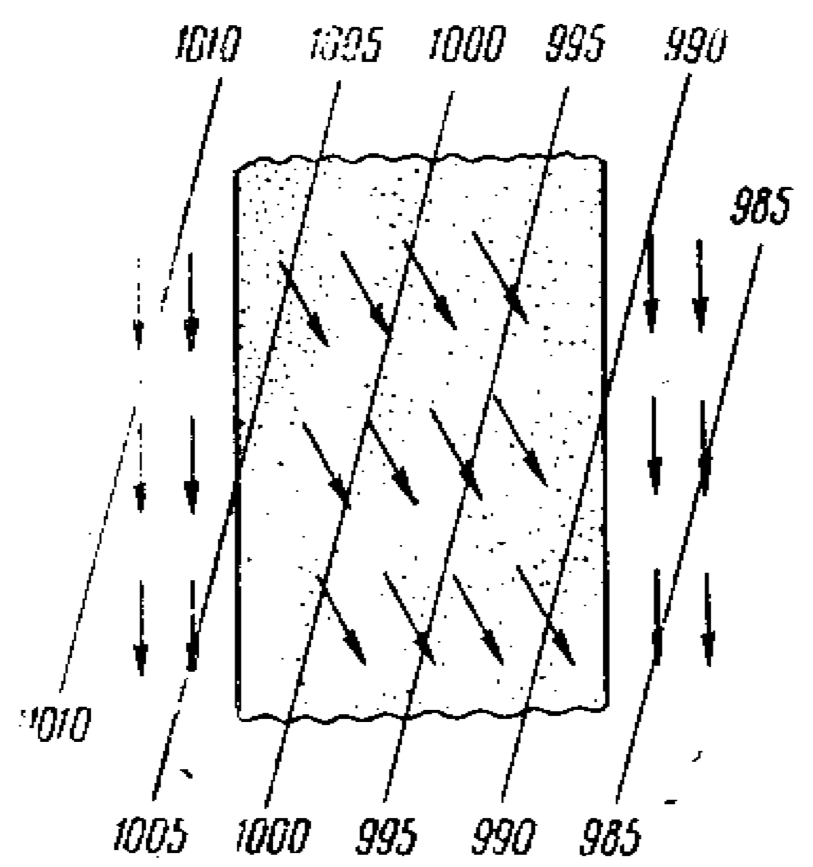
\includegraphics[scale=0.2]{02_coast_effect.png}
   \caption{Береговой эффект}
   \label{fig:02_coast_effect}
\end{figure*}

Всякое препятствие, стоящее на пути воздушного потока, отклоняет его,
и он либо обтекает препятствие с боков, либо перетекает через него
сверху. При горизонтальном обтекании ветер усиливается у мысов,
оконечностей островов и т.\,п., так как линии тока в таких местах
сближаются. Это усиление ветра называется \textbf{угловым
  эффектом}\index{угловой эффект}. Если мыс или остров остаётся справа
от направления линии тока, то ветер будет особенно сильным. Примером
является \textbf{бакинский норд}\index{бакинский норд} "--- ветер
северных направлений у Апшеронского полуострова на Каспийском море.

Существенное усиление ветра наблюдается в проливах с высокими
берегами, причём в них преобладают ветры, дующие вдоль пролива.  За
препятствиями скорость ветра уменьшается, и там образуется ветровая
тень. Этим объясняется известный факт, что в заливах, бухтах и фьордах
ветер значительно слабее, чем в открытом море.

\section{Изобары}
\label{sec:isobars}

\textbf{Изобарами}\index{изобары} называются линии, соединяющие на карте точки с равным атмосферным давлением.

\section{Барическое поле}
\label{sec:baric_field}

\textbf{Барическое поле}\index{барическое поле} "--- распределение давлений на каком-либо горизонтальном уровне.

\section{Формы барического рельефа}
\label{sec:baric_relief}

\textbf{Формы барического рельефа}\index{барического рельефа форма}
"--- системы расположения изобар, характеризующие тип падения или
повышения давления. Различают следующие формы барического рельефа:
\textbf{циклон}, \textbf{ложбина}, \textbf{антициклон},
\textbf{отрог}, \textbf{гребень} или \textbf{клин},
\textbf{седловина}.

\section{Барическая тенденция}
\label{sec:baric_tendency}

\textbf{Барическая тенденция}\index{барическая тенденция} "--- это
величина изменения давления в течении трёх часов перед последним
наблюдением.

\section{Барический закон ветра}
\label{sec:baric_wind_law}

\textbf{Барический закон ветра}\index{барический закон ветра} "---
если встать спиной к ветру, то в северном полушарии низкое давление
находится слева, а высокое "--- справа от направления ветра. В южном
полушарии "--- наоборот.

\section{Циклоны}

\subsection{Циклон}
\label{sec:cyclon}

\begin{figure*}[htb]
   \centering
   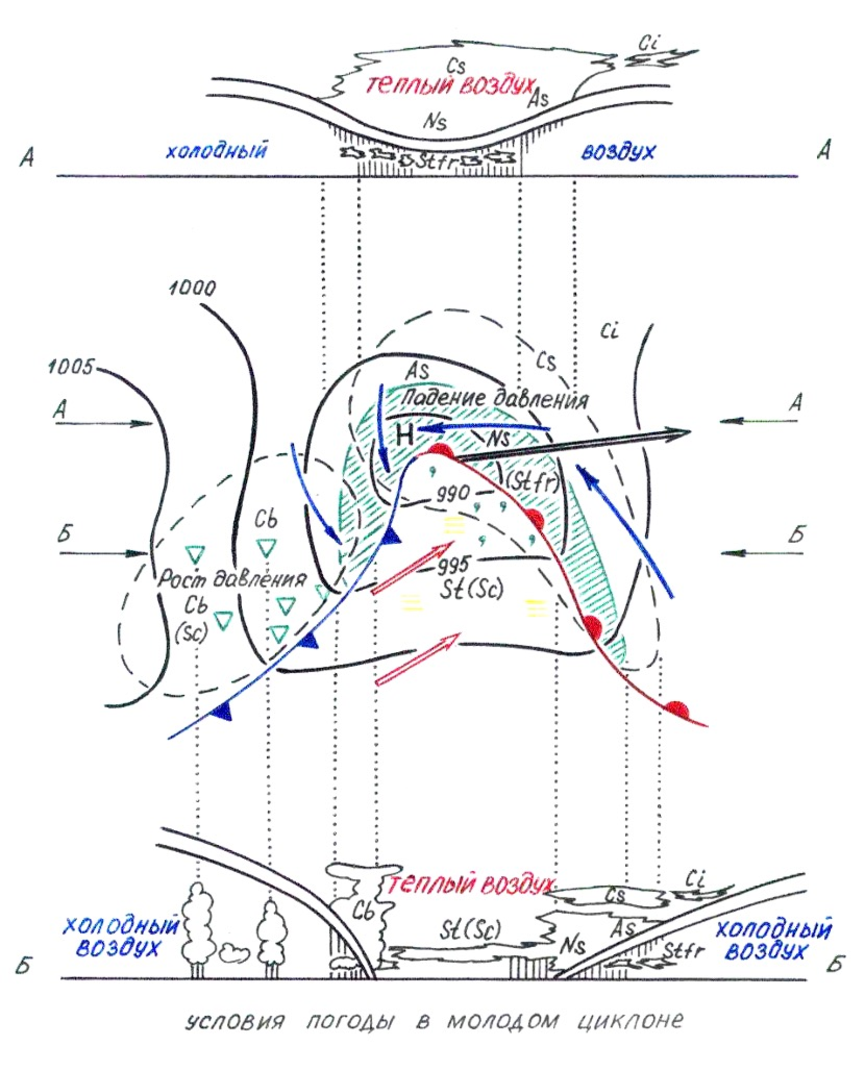
\includegraphics[scale=1.0]{03_cyclon.pdf}
   \caption{Условия погоды в молодом циклоне}
   \label{fig:03_cyclon}
\end{figure*}


\textbf{Циклон}\index{циклон} "--- вихреобразное возмущение в
атмосфере с понижающимся давлением к центру. Характеризуется системой
ветров, дующих против часовой стрелки в северном полушарии и по
часовой стрелке в южном полушарии. Циклон зарождается, когда область
пониженного давления возникает на границе двух масс воздуха разной
температуры. В циклонах два фронта "--- холодный и тёплый. Стадии
развития циклона: волна, волновой циклон, окклюзия или замыкание,
вихрь.

Стадия молодого циклона (рис.~\ref{fig:03_cyclon}) характеризуется
наличием тёплого сектора, т.\,е. сектора в южной части депрессии с
тёплым воздухом и ограниченного спереди тёплым фронтом, сзади "---
холодным. Холодный фронт в развивающемся циклоне движется быстрее
тёплого. Стадия молодого циклона продолжается до тех пор, пока в
центре циклона у земной поверхности остаётся тёплый
воздух. Продолжительность этой студии в среднем 12\otdo24~ч. В молодом
циклоне можно выделить три зоны, резко различающиеся по условиям
погоды.

\subsection{Антициклон}
\label{sec:anticyclon}

\begin{figure*}[htb]
   \centering
   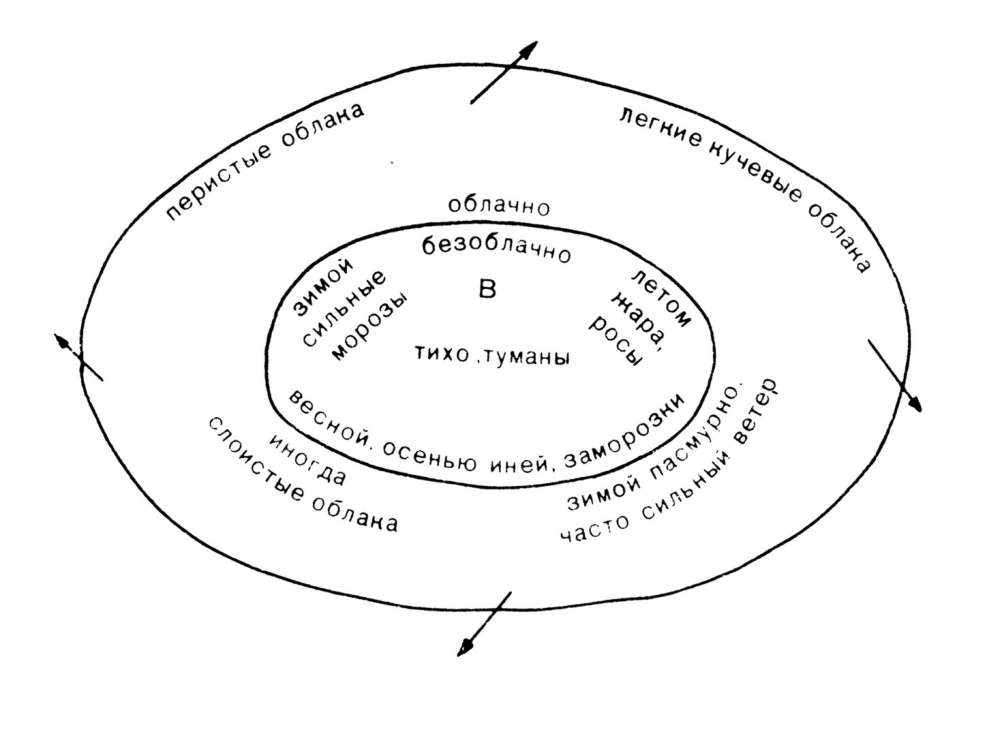
\includegraphics[scale=1.0]{04_anticyclon.pdf}
   \caption{Антициклон}
   \label{fig:04_anticyclon}
\end{figure*}

\textbf{Антициклон}\index{антициклон} "--- вихреобразное возмущение в
атмосфере с повышенным давлением в центре; область повышенного
атмосферного давления, состоящая из однородной воздушной массы
вращающейся по часовой стрелке в севером полушарии
(рис.~\ref{fig:04_anticyclon} и против часовой стрелки в южном
полушарии.

\section{Фронты}

\subsection{Атмосферный фронт}
\label{sec:front}

\textbf{Атмосферный фронт}\index{атмосферный фронт} "--- сравнительно
узкая (несколько километров) переходная зона между двумя воздушными
массами.

Если воздушный поток направлен от тёплой воздушной массы к холодной,
то и фронт перемещается в этом направлении, такой фронт называется
\textbf{тёплым}\index{фронт!тёплый}.

\begin{figure*}[htb]
   \centering
   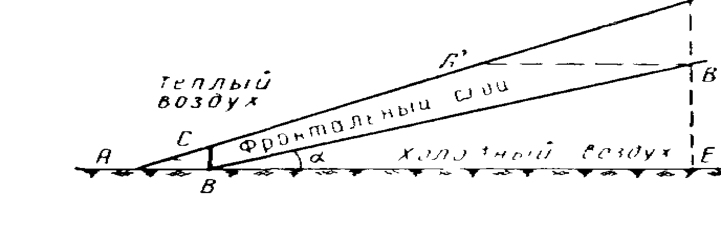
\includegraphics[scale=1.0]{05_vertical_front.pdf}
   \caption{Вертикальный разрез фронтального слоя}
   \label{fig:05_vertical_front}
\end{figure*}

Ширина фронтального слоя (рис.~\ref{fig:05_vertical_front} в приводном
(приземном) слое (отрезок $AB$) наименьшая: от нескольких до десятков
километров, а на высоте 3\otdo5~км ($A'B'$) может достигать
300~км. В верхней половине тропосферы ширина фронтальной зоны может
быть ещё больше. Вертикальная мощность слоя ($BC$ и $B'P$) обычно не
превышает 1~км. Горизонтальная проекция фронта $AE$ составляет
100\otdo1000~км, а его высота $EP$ "--- от 1 до 10~км.

Обычно толщиной фронтального слоя пренебрегают и считают, что фронт
"--- поверхность, которую называют фронтальной.

Различают следующие фронты: \textbf{основные}\index{фронт!основной}
(их называют тропосферными\index{фронт!тропосферный}, или
высокими\index{фронт!высокий}), \textbf{вторичные}\index{фронт!вторичный}
(приземные\index{фронт!приземный}, низкие\index{фронт!низкий}) и
\textbf{верхние}\index{фронт!верхний}.

Основными называются фронты, имеющие большую горизонтальную
(несколько тысяч километров) и вертикальную протяжённость. Эти фронты
разделяют воздушные массы, существенно отличающиеся по своим
свойствам.

Скачок температуры при переходе через линию основного фронта на
приземной карте обычно превышает 5\grC.

Вторичными называются фронты небольшой горизонтальной протяжённости,
(несколько сот километров).  Они разделяют различные порции одной и
той же воздушной массы. Высотная фронтальная зона со вторичными
фронтами не связана.

Верхними называются фронты, которые могут быть прослежены на картах
барической топографии, но не выявляются на приземных картах погоды.

Каждый основной фронт неоднороден по своим свойствам на всех
участках. Одни участки смещаются в сторону тёплой воздушной массы,
другие \--— в сторону холодной, третьи "--- малоподвижны. Поэтому фронты
классифицируются по ряду дополнительных признаков.

\subsection{Тёплый фронт}
\label{sec:warm_front}\index{фронт!тёплый}

\textbf{Тёплым} называются участки основного фронта, перемещающиеся в сторону
относительно холодной воздушной массы. За тёплым фронтом перемещается
тёплая воздушная масса.

\begin{figure*}[htb]
   \centering
   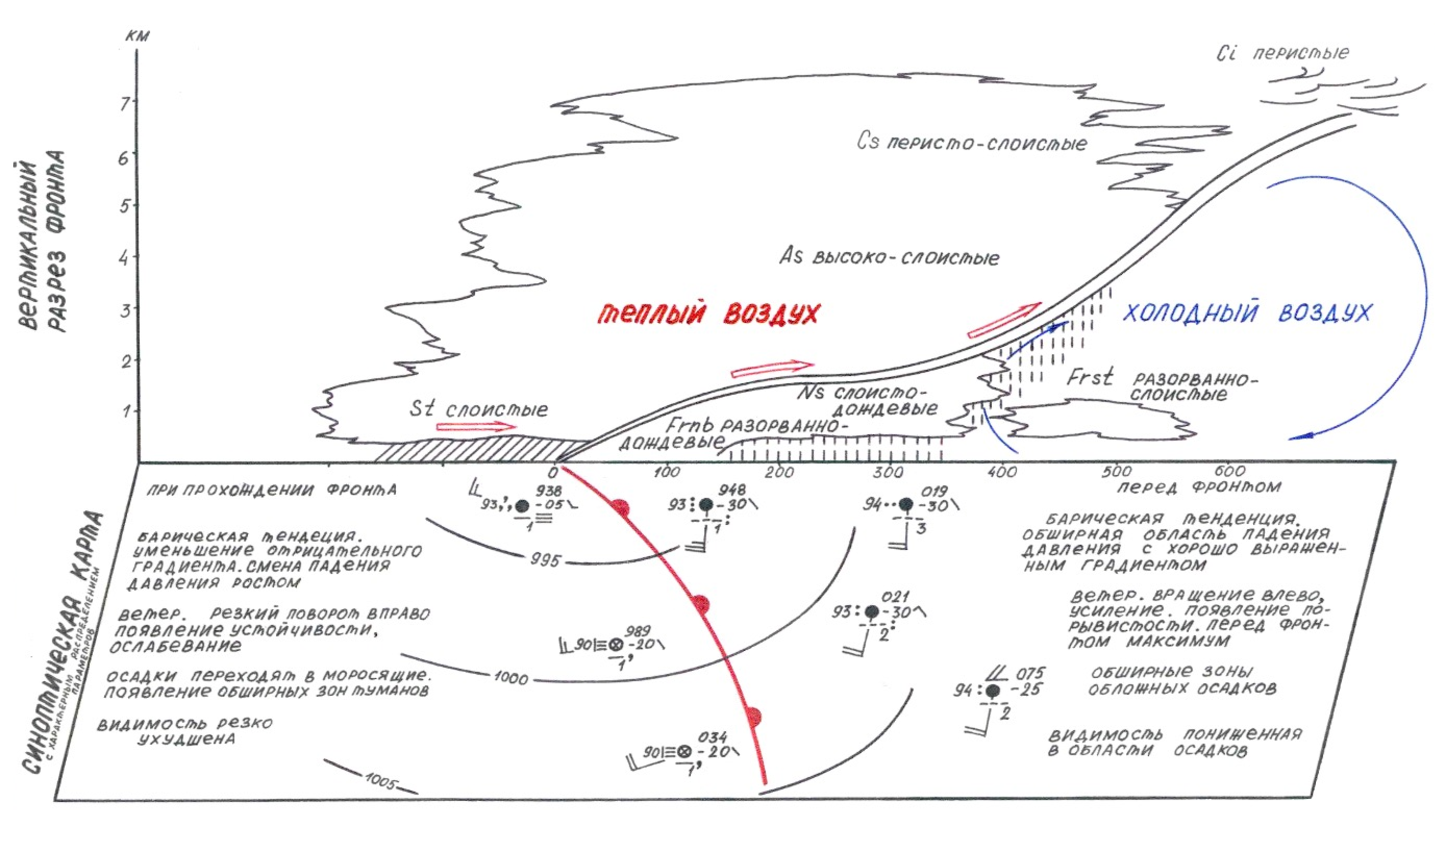
\includegraphics[scale=0.7]{06_warm_front.pdf}
   \caption{Тёплый фронт}
   \label{fig:06_warm_front}
\end{figure*}

Если фронт тёплый, то тёплый воздух натекает на холодный, поднимается
вверх над клином холодного воздуха и адиабатически
охлаждается. Содержащийся в нем водяной пар достигает насыщения и
конденсируется, образуя мощную облачную систему, состоящую из
слоисто-дождевых (\textit{Ns}), высоко-слоистых (\textit{Аs}) и
перисто-слоистых (\textit{Cs}) облаков, постепенно переходящих одни в
другие и образующих вместе как бы гигантский клинообразный массив,
сужающийся вперёд. Нижняя граница этого облачного массива
приблизительно совпадает с верхней границей фронтального слоя. Впереди
и несколько выше фронтальной поверхности обычно возникают перистые
облака (\textit{Ci}). Под поверхностью фронта в массах холодного
воздуха обычно образуются разорванно-слоистые (\textit{Frst}) облака.

На рис.~\ref{fig:06_warm_front} приведена схема вертикального строения
облачной системы тёплого фронта. Однако в каждом конкретном случае
строение облачной системы тёплых фронтов может существенно отличаться
от этой схемы.

Перед линией тёплого фронта образуется зона обложных
осадков\index{зона обложных осадков}, наибольшая ширина которой при
дожде достигает 300~км., а при снеге "--- 400~км. Это связано с тем,
что снег из высоко-слоистых облаков чаще достигает земной поверхности,
в то время как дождь в летнее время обычно при падении испаряется и до
земной поверхности не доходит. Внутри области осадков часто
наблюдается туман, обусловленный притоком водяного пара в холодный
воздух за счёт испарения осадков, а также адиабатическим охлаждением
воздуха в связи с падением давления. Ширина зоны тумана может
достигать 100\otdo200~км. Предфронтальный туман тёплого фронта чаще
всего образуется в холодное время года. Плохая видимость и сильный
ветер являются основными трудностями, которые могут встретиться при
пересечении тёплого фронта. Кроме того, зимой здесь возможно
обледенение судна.

После прохождения тёплого фронта наступает потепление. Вся система
облачности находится перед тёплым фронтом, поэтому по характеру
изменения облачности можно судить о приближении тёплого фронта.

При появлении перистых облаков начинается сначала медленное, а затем
постепенно ускоряющееся падение давления, которое прекращается
незадолго до прохождения линии фронта; после её прохождения давление
остаётся неизменным или медленно понижается, а иногда растёт.

Изменение скорости и направления ветра также является хорошим
признаком приближения тёплого фронта. По мере падения давления
скорость ветра постепенно увеличивается, достигая наибольшей величины
перед прохождением фронта. Направление ветра медленно отклоняется
влево, а в момент прохождения линии фронта резко поворачивает вправо
(в северном полушарии).

\subsection{Холодный фронт}
\label{sec:cold_front}\index{фронт!холодный}

\textbf{Холодными} называются участки основного фронта, перемещающиеся в
сторону относительно тёплой воздушной массы. За холодным фронтом
перемещается холодная воздушная масса.

Если воздушный поток направлен от холодной воздушной массы к более
тёплой, то такой фронт называется холодным. Отставание нижних слоев
воздуха от верхних под влиянием трения о земную поверхность приводит к
тому, что верхние слои обрушиваются вниз: холодный фронт приобретает
форму катящегося вала. Вытесняемый прямо вверх тёплый воздух быстро
поднимается и образует гряду тёмных туч "--- кучево-дождевых
облаков. В зависимости от скорости перемещения холодного воздуха
различают холодные фронты \textit{первого} (скорость передвижения
невелика, рис.~\ref{fig:07_cold_front_1}) и \textit{второго} рода
(рис.\ref{fig:08_cold_front_2}).

Структура холодных фронтов различается в зависимости от того, быстро
или медленно они движутся.

По этой причине различают: холодные фронты 1-го
рода\index{фронт!холодный 1-го рода} "--- медленно движущиеся фронты,
у которых облачность и осадки располагаются в основном за линией
холодные фронты 2-го рода\index{фронт!холодный 2-города} "--- быстро
движущиеся фронты, у которых облачность и осадки расположены в
основном перед линией фронта.

Холодные фронты 2-го рода наблюдаются в центральной части
циклона, а 1-го рода "--- на его периферии.

При холодном фронте 1-го рода происходит вытеснение масс тёплого
воздуха вторгающимся под него клином холодного воздуха. Здесь характер
облачности представляет собой зеркальное изображение облачности
тёплого фронта. Непосредственно перед линией фронта возникает
кучево-дождевые облака (\textit{Cb}), из которых выпадают ливневые осадки,
сопровождаемые грозами. Ширина зоны ливневой облачности "--- несколько
десятков километров.

\begin{figure*}[htb]
   \centering
   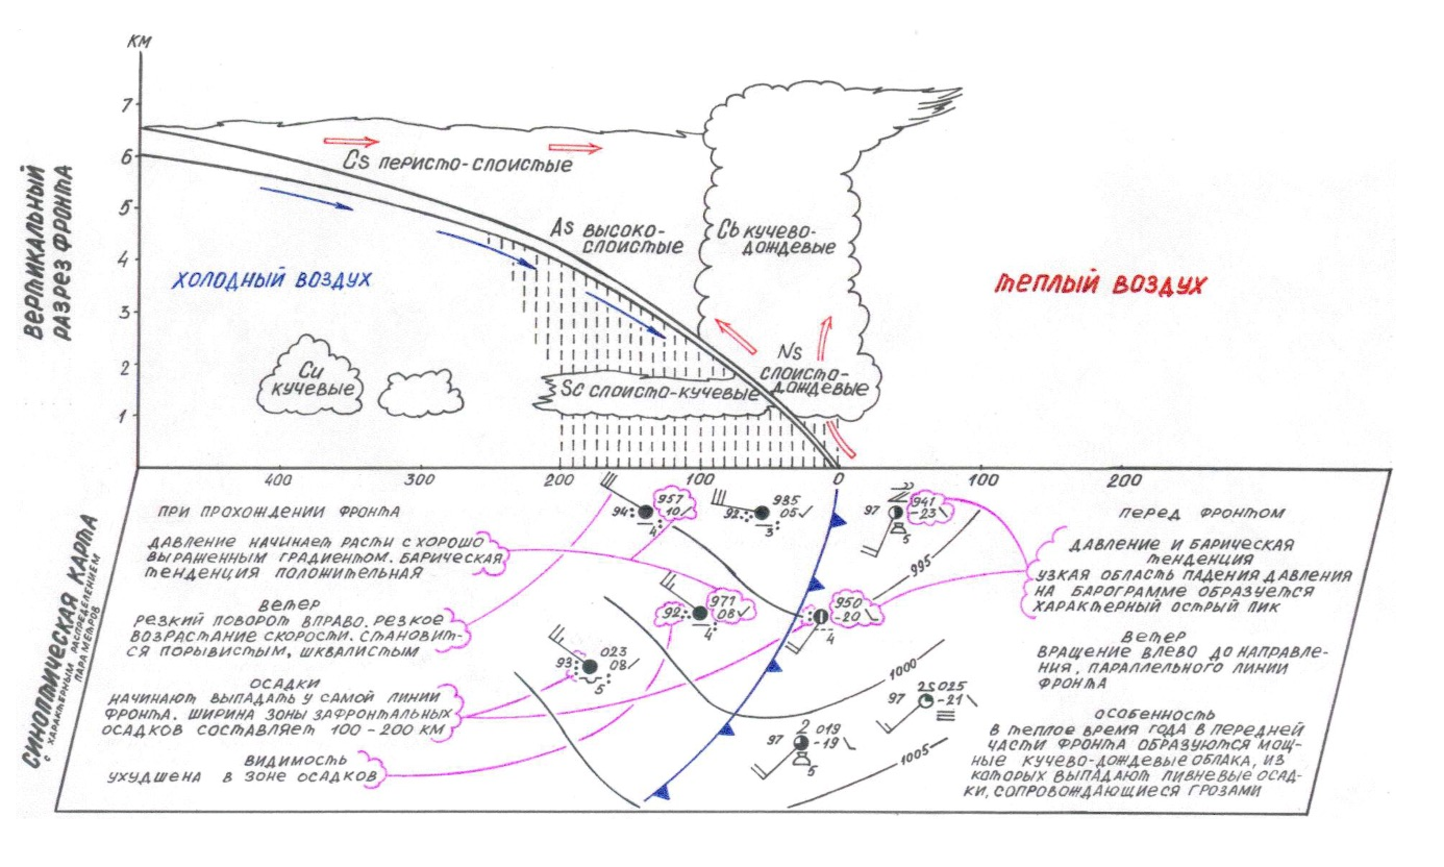
\includegraphics[scale=0.7]{07_cold_front_1.pdf}
   \caption{Холодный фронт 1-го рода}
   \label{fig:07_cold_front_1}
\end{figure*}

Облачная система \textit{Ns-As} с обложными осадками располагается за
линией фронта. Ширина зоны облачности, её мощность и, соответственно,
ширина зоны осадков примерно вдвое меньше, чем У тёплого фронта.

Таким образом, в отличие от тёплого фронта система облачности
холодного воздуха 1-го рода не позволяет заранее обнаружить его
приближение.

Холодный фронт 2-го рода отличается тем, что быстрое перемещение вала
холодного воздуха вызывает перед линией фронта бурный подъём
оттесняемого тёплого воздуха, а нисходящие движения воздушных потоков
препятствуют распространению облачной системы непосредственно за
линией фронта.

\begin{figure*}[htb]
   \centering
   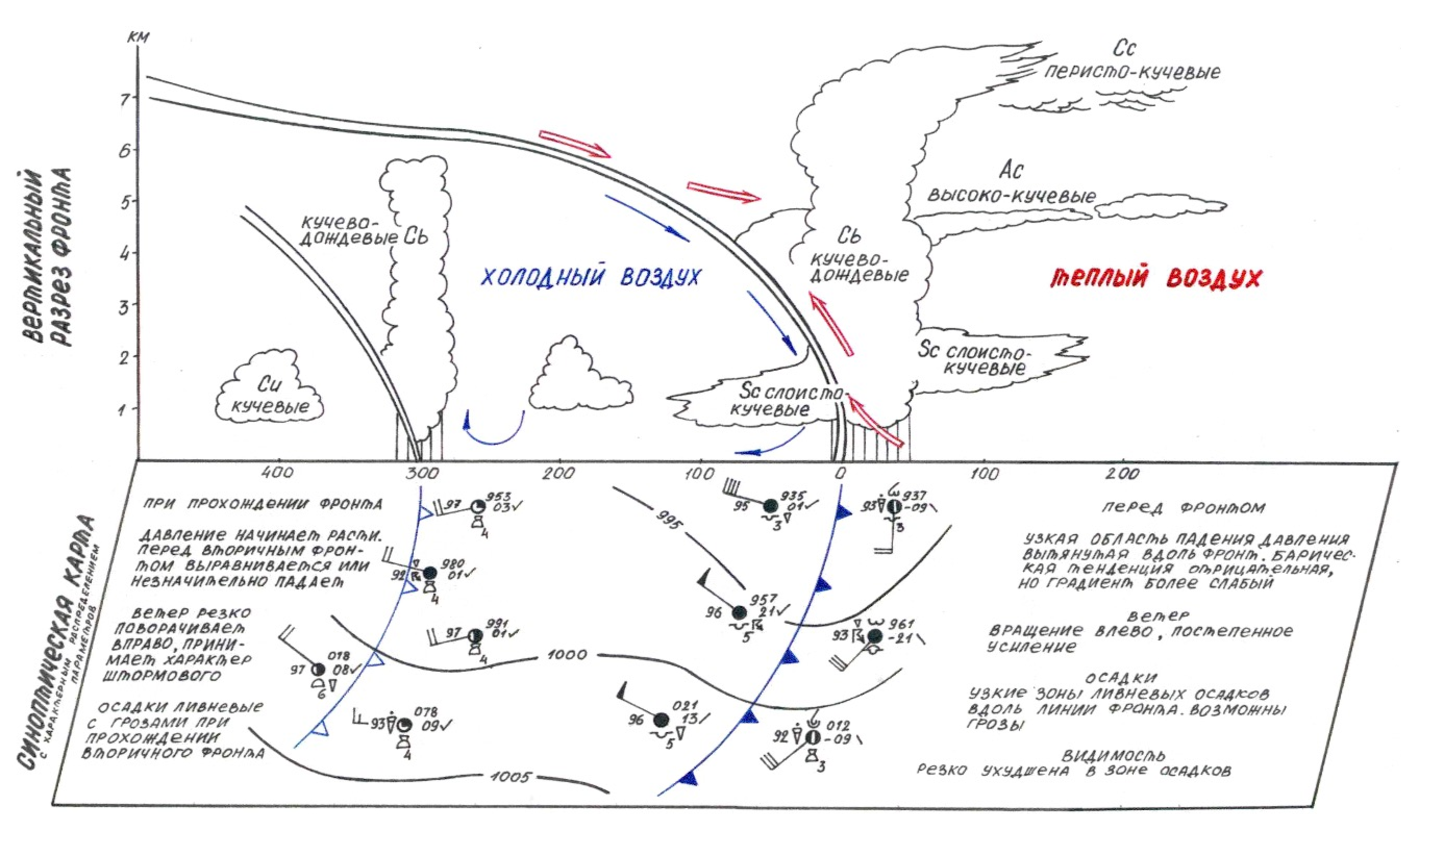
\includegraphics[scale=0.7]{08_cold_front_2.pdf}
   \caption{Холодный фронт 2-го рода}
   \label{fig:08_cold_front_2}
\end{figure*}

Возникающая облачная система представляет собой в основном вал мощных
облаков \textit{Cb}. При их растекании в небольшом количестве могут
образоваться \textit{Ci}, \textit{Cc}, \textit{Ac} и \textit{Sc}, а
под ними, в зоне выпадающих ливневых осадков, обычно наблюдаются
\textit{Cb} или \textit{Cu fra} (\textit{Cu fra} — разорванные
кучевые) плохой погоды.  На высотах 4\otdo5~км восходящий поток
адиабатически охлаждённого влажного воздуха встречается с нисходящим
потоком адиабатически нагретого сухого воздуха. В результате
образуется верхний вторичный фронт, под которым вал облаков
\textit{Cb} вытягивается вперёд. Передний его край, имеющий характер
\textit{Sc}, может постепенно разделиться на гряды чечевицеобразных
облаков \textit{Ac}. Эти облака выносятся вперёд от линии фронта на
200\otdo300 км и их обнаружение является надёжным предупреждением о
приближении холодного фронта 2-го рода.

Позади линии фронта в холодной массе воздуха наблюдаются нисходящие
движения воздуха, особенно значительные в передней части клина
холодного воздуха. Поэтому внутримассовые облака здесь не
возникают. Вскоре после прохождения линии фронта наступает быстрое
прояснение, вплоть до полного; лишь через несколько часов, когда
нисходящие движения затухнут и фронтальная поверхность достаточно
приподнимется, могут появиться свойственные холодной неустойчивой
массе конвективные облака и ливневые осадки.

Ливневые осадки при прохождении холодного фронта 2-го рода
непродолжительны (от нескольких минут до 1~ч), поскольку ширина зоны
осадков небольшая, а скорость перемещения фронта значительная.

В вале кучево-дождевых облаков холодного фронта 2-го рода иногда
встречаются разрывы или менее развитая облачность нижнего и среднего
ярусов. На отдельных участках фронта развивается грозовая
деятельность, которая, затухнув на одних участках, может появиться на
соседних.

Направление ветра при прохождении холодных фронтов обоих родов
изменяется так же, как и в случае тёплого фронта, но поворот вправо
(в северном полушарии) в момент прохождения линии холодного фронта "---
более значительный и резкий. Одновременно резко усиливается скорость
ветра.

При приближении холодного фронта наблюдается непродолжительное,
обычно слабое, но постепенно ускоряющееся падение давления. Тотчас по
прохождении линии фронта начинается рост давления, обусловленный
заменой тёплого воздуха холодным.

Температура воздуха после прохождения линии фронта понижается. Скачок
температуры зависит от характера сменяющихся масс.

Холодным фронтам обоих родов свойственны предфронтальные шквалы. Для
воздуха за холодным фронтом характерно нисходящее движение, которое
становится особенно интенсивным в передней части холодного клина, где
благодаря трению создаётся крутой наклон фронтальной
поверхности. Холодный воздух, обрушиваясь вниз, как бы перекатывается
вперёд, подобно гусеницам танка, причём скорость его продвижения
нормально к линии фронта во всех случаях оказывается больше, чем
соответствующая составляющая скорости тёплого воздуха в нижних
слоях. Обрушивание холодного воздуха приводит к вытеснению вверх
тёплого воздуха и к возникновению вдоль фронта вихря с горизонтальной
осью; с этим вихрем и связаны явления фронтальных шквалов.

Особенно интенсивное нисходящее движение имеет место в голове
холодного воздуха. Опускающийся с высоты нескольких километров, этот
воздух адиабатически нагревается, и благодаря этому скачок температуры
вдоль фронта сглаживается. В некоторых случаях внутри холодного клина
возникает вторичный холодный фронт, отделяющий нагревшийся воздух
<<головы>> от воздуха, лежащего дальше от линии фронта и не
захваченного в такой степени нисходящим движением.

Этот второй холодный фронт идёт на расстоянии нескольких километров за
размывшимся основным фронтом. При его прохождении наблюдается скачок
температуры, ветры и шквалы, но облачной системы он не имеет. Это
явление называют раздвоением холодного фронта.  В барических ложбинах
в тылу циклона обычно формируются вторичные холодные фронты. Причины
их образования будут рассмотрены ниже. Они имеют систему облаков,
сходную с системой облаков холодного фронта 2-го рода, однако
вертикальная протяжённость облаков меньше протяжённости облаков
основных холодных фронтов. В отдельных случаях может быть несколько
ложбин и вторичных фронтов.  Малоподвижными (стационарными) называются
участки основного фронта, не претерпевающие существенного
перемещения.

В циклоне холодный фронт перемещается несколько быстрее тёплого. С
течением времени происходит их сближение, а затем и слияние,
начинающееся близ центра циклона. Такой фронт, образовавшийся в
результате слияния холодного и тёплого фронтов, называется
\textbf{фронтом окклюзии}\index{фронт!окклюзии} (сомкнутым
фронтом\index{фронт!сомкнутый}).

Если холодный фронт догоняет идущий впереди него тёплый фронт;
холодный воздух, расположенный за холодным фронтом, смыкается с
холодным воздухом, расположенным перед тёплым фронтом, то такой
процесс называется окклюзией (окклюдированием) циклона, а сложный
фронт называется фронтом окклюзии. Скорость ветра в циклоне достигает
максимума непосредственно после начала окклюзии, циклон находится в
стадии максимального развития. В последующем наступает стадия
заполнения циклона. Атмосферное давление начинает расти, скорость
ветра уменьшаться.

\subsection{Фронты окклюзии}
\label{sec:ocl_front}

\textbf{Фронты окклюзии}\index{фронт!окклюзии} соединяют в себе черты
тёплого и холодного фронтов, но часто выражены менее резко.  В системе
фронтов окклюзии взаимодействуют три воздушные массы, из которых
наиболее тёплая уже не соприкасается с земной поверхностью. Поэтому,
помимо приземной линии, имеется линия верхнего фронта. При
образовании этого фронта может быть три случая:
\textit{нейтральная}\index{фронт!окклюзии!нейтральной},
\textit{тёплая}\index{фронт!окклюзии!тёплой} и
\textit{холодная}\index{фронт!окклюзии!холодной} окклюзия.

\textbf{Нейтральная}\index{фронт!окклюзии!нейтральной} имеет место,
когда массы холодного воздуха, движущиеся за холодным фронтом, имеют
одинаковую температуру с холодным воздухом, перемещающимся впереди
тёплого фронта. В момент смыкания холодных масс фронт отрывается от
земной поверхности и возникает верхний фронт. Характер облачности при
этом будет определяться системами облачности как тёплого, так и
холодного фронтов. В последующем будет происходить размывание
облачности и дальнейшее вытеснение тёплого воздуха вверх. Случай
нейтральной окклюзии очень редок, так как обычно температуры
отступающего и наступающего холодного воздуха неодинаковы. Иногда по
распределению температуры трудно судить о типе фронта окклюзии, в
связи с чем и было введено понятие окклюзии без уточнения. Часто
используются также термины: <<окклюзия по типу тёплого фронта>> и
<<окклюзия по типу холодного фронта>>.

Если холодный воздух за холодным фронтом оказывается теплее холодного
воздуха перед тёплым фронтом, то при прохождении линии фронта у
поверхности Земли будет отмечаться некоторое повышение температуры, и
в этом случае окклюзия называется \textbf{тёплой}
(рис.~\ref{fig:10_warm_ocl_front}). Характер облачности в начальный
момент одинаков с характером облачности при нейтральной окклюзии. В
последующем, в связи с тем, что холодный фронт перемещается быстрее
тёплого фронта, менее холодный воздух будет натекать на более
холодный. Массы тёплого воздуха вытесняются вверх, и образуются две
зоны раздела: верхний холодный и нижний тёплый фронты. По своим
внешним признакам тёплый фронт окклюзии сходен с тёплым фронтом. Все
признаки, относящиеся к тёплому фронту, справедливы и для тёплого
фронта окклюзии, однако они выражены значительно слабее.

\begin{figure*}[htb]
   \centering
   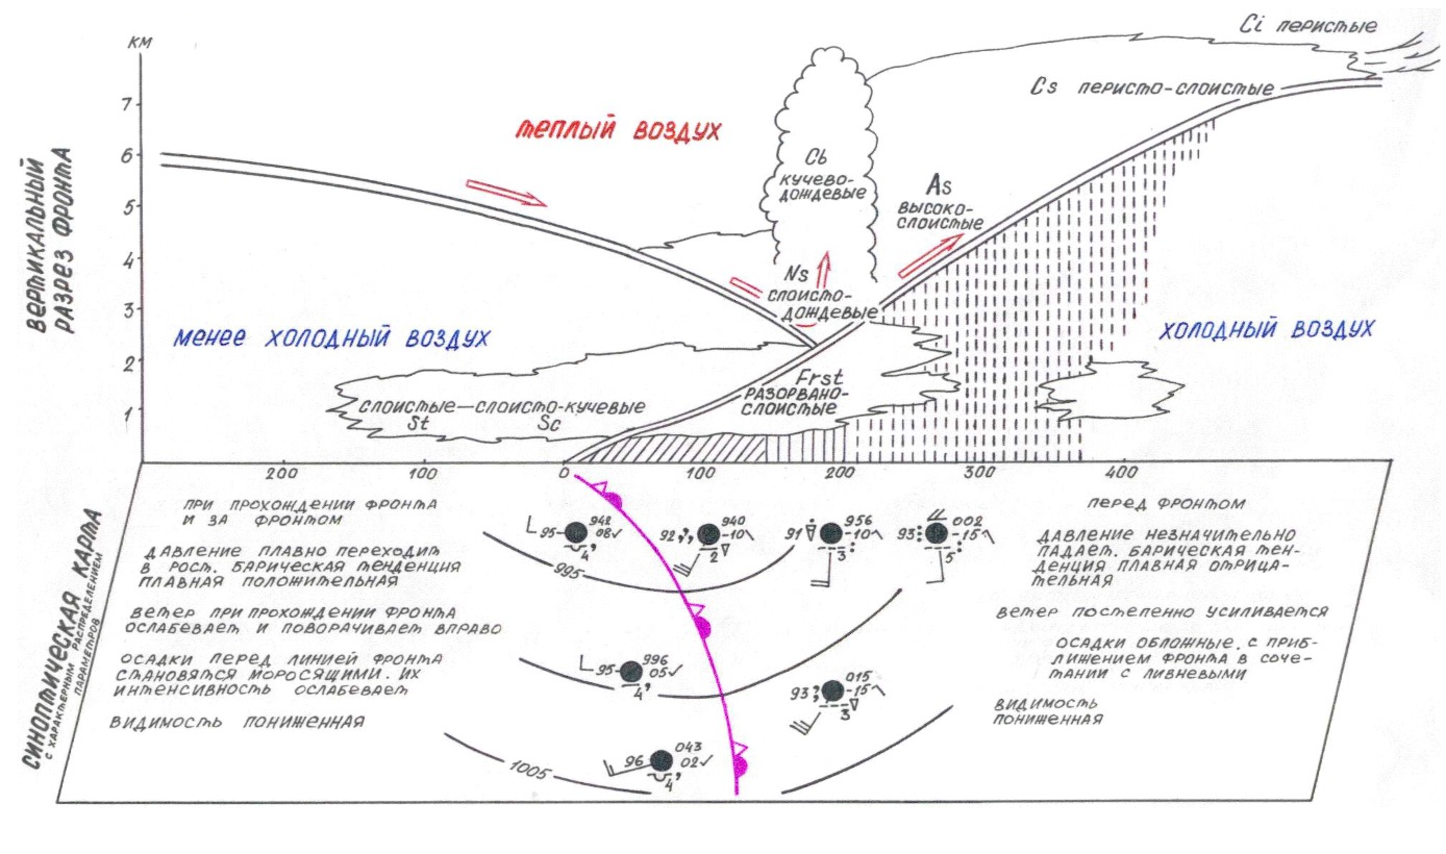
\includegraphics[scale=0.7]{10_warm_ocl_front.pdf}
   \caption{Фронт тёплой окклюзии}
   \label{fig:10_warm_ocl_front}
\end{figure*}

Если температура холодного воздуха за наступающим холодным фронтом
ниже температуры отступающего холодного воздуха перед тёплым фронтом,
то при прохождении линии фронта у поверхности Земли происходит
похолодание, и в этом случае окклюзия называется \textbf{холодной}
(рис.~\ref{fig:09_cold_ocl_front}). По всем внешним признакам холодный
фронт окклюзии сходен с холодным фронтом 1-го рода. Как и в предыдущем
случае, здесь также возникают две зоны раздела: верхний тёплый и
нижний холодный фронты.

\begin{figure*}[htb]
   \centering
   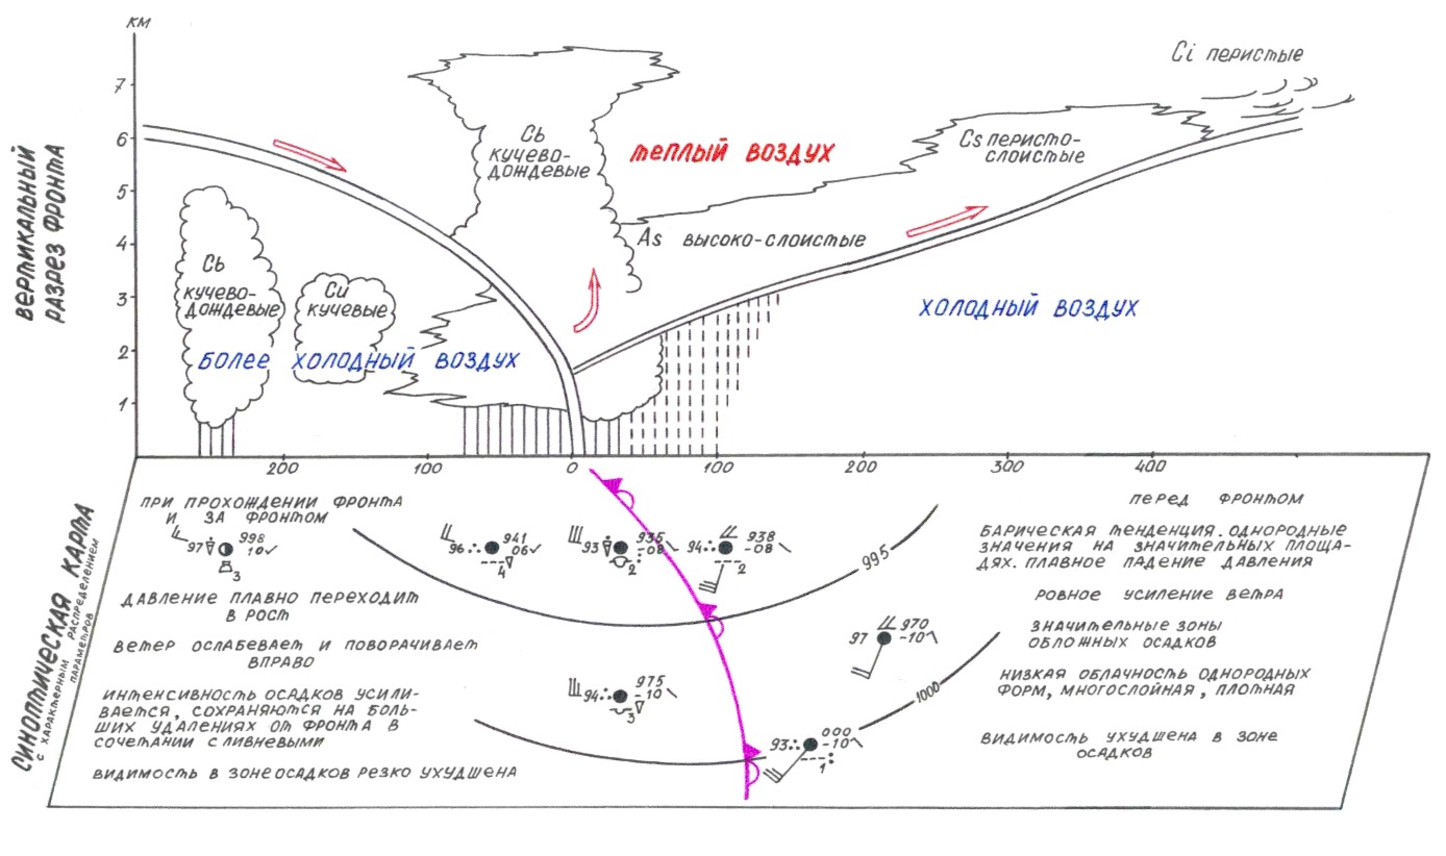
\includegraphics[scale=0.7]{09_cold_ocl_front.pdf}
   \caption{Фронт холодной окклюзии}
   \label{fig:09_cold_ocl_front}
\end{figure*}

Поскольку, как правило, верхний фронт расположен близко от приземного,
то на картах погоды практически их разграничить невозможно.

При прохождении фронта окклюзии направление ветра в северном полушарии
меняется по часовой стрелке, как и при прохождении тёплого или
холодного фронта.

Как при тёплой, так и при холодной окклюзии при небольшом контрасте
температур в массах холодного воздуха и при условии, что этот контраст
не усиливается, происходит размывание фронтов окклюзии. Если же
контраст температур достаточно большой или он усиливается, то
развивается облачность по типу тёплого или холодного фронтов.

В зависимости от соотношения температур воздуха по обе стороны фронта
окклюзии и направления его перемещения различают тёплые и холодные
фронты окклюзии. При одинаковой температуре по обе стороны фронт
окклюзии называется нейтральным.

По географической классификации различают следующие главные атмосферные фронты:
\textbf{арктический}\index{фронт!арктический}, разделяющий массы арктического и полярного (умеренного) воздуха;
\textbf{полярный}\index{фронт!полярный} (умеренный), разделяющий массы полярного (умеренного) и тропического воздуха;
\textbf{тропический}\index{фронт!тропический}, разделяющий массы тропического и экваториального воздуха.

\begin{figure*}[htb]
   \centering
   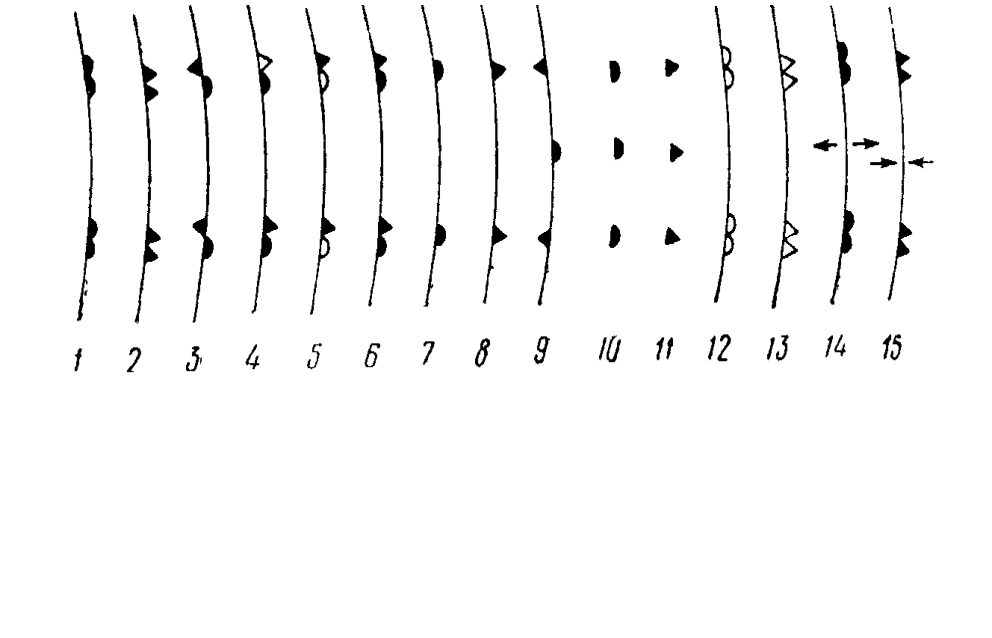
\includegraphics[scale=1]{11_fronts_marks.pdf}
   \caption{Фронт холодной окклюзии}
   \label{fig:fronts_marks}
   \small
   \begin{enumerate*}[itemjoin={{; }}, label={\arabic*~\--}]
   \item тёплый
   \item холодный
   \item малоподвижный
   \item тёплой окклюзии
   \item холодной окклюзии % 5
   \item нейтральной окклюзии
   \item тёплый размытый
   \item холодный размытый
   \item малоподвижный размытый
   \item тёплый вторичный % 10
   \item холодный вторичный
   \item тёплый верхний
   \item холодный верхний
   \item тёплый размывающийся
   \item холодный обостряющийся %15
   \end{enumerate*}
\end{figure*}

На рис.~\ref{fig:fronts_marks} показаны условные обозначения фронтов,
применяемые на фототелеграфных картах погоды.

Следует подчеркнуть, что рассмотренная схема отражает только главные
черты развития циклона. В действительности могут быть значительные
отклонения от этой схемы.

\subsection{Образование и размывание фронтов}
\label{sec:makes_fronts}

Фронты любого типа могут быть в одних случаях резко выраженными, или
\textbf{обострёнными}\index{фронт!обострение}, в других случаях "--- слабо
выраженными, или \textbf{размытыми}\index{фронт!размытие}.

Если фронт \textit{обострённый}, то при переходе через его линию резко
изменяются температура воздуха и другие метеорологические элементы,
если \textit{размыт} \--— температура и другие метеорологические
элементы меняются постепенно.

Процессы образования и обострения фронтов называются
\textbf{фронтогенезом}\index{фронтогенез}, а процессы размывания
фронтов "--- \textbf{фронтолизом}\index{фронтолиз}. Эти процессы
наблюдаются непрерывно, подобно тому, как непрерывно формируются и
трансформируются воздушные массы.

Для образования фронта необходимо существование хотя бы небольшого
горизонтального градиента температуры и такого поля ветра, под
действием которого этот градиент значительно увеличился бы в некоторой
узкой полосе.

Особую роль в образовании и размывании фронтов играют \textit{барические
седловины} и связанные с ними \textit{деформационные поля ветра}. Если изотермы
в переходной зоне между соседними воздушными массами располагаются
параллельно оси растяжения или под углом менее 45\gr к ней, то в
деформационном поле происходит их сближение и горизонтальный
температурный градиент увеличивается. Наоборот, при расположении
изотерм параллельно оси сжатия или под углом менее 45\gr к ней
расстояние между ними увеличивается, и если уже сформированный фронт
попадёт под такое поле, произойдёт размывание фронта.

\subsection{Профиль фронтальной поверхности}
\label{sec:frontal_surface_profile}

Угол наклона \textbf{фронтальной поверхности} зависит от разности
температуры и скорости ветра тёплой и холодной воздушной массы. На
экваторе фронты не пересекаются с земной поверхностью, а превращаются
в горизонтальные слои инверсии. Следует отметить, что на величину
наклона поверхности тёплого и холодного фронтов некоторое влияние
оказывает трение воздуха о земную поверхность. В пределах слоя трения
скорость движения фронтальной поверхности с высотой увеличивается, а
выше уровня трения почти не изменяется. Это по-разному влияет на
профиль поверхности тёплого и холодного фронтов. На рисунке
~\ref{fig:firction_sufrace_profile}\textit{a} линия \textit{I}
показывает первоначальное положение стационарного фронта с одинаковым
наклоном на всех уровнях.

\begin{figure*}[htb]
   \centering
   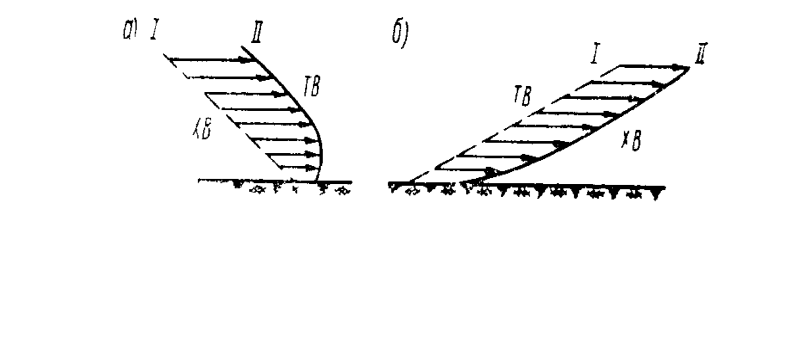
\includegraphics[scale=1]{12_friction_surface_profile.pdf}
   \caption[Влияние трения на профиль поверхностей]{Влияние трения на профиль поверхностей:}
   \label{fig:firction_sufrace_profile}
   \small
   \begin{enumerate*}[itemjoin={{; }}, label={}, after={{; }}]
   \item а "--- холодного фронта
   \item б "--- тёплого фронта
   \end{enumerate*}
   \begin{enumerate*}[itemjoin={{; }}, label={\Roman* "--- }]
   \item стационарный
   \item движущийся фронт
   \end{enumerate*}
\end{figure*}

Когда фронт начал смещаться как тёплый, в том слое, где скорость
движения с высотой возрастает, фронтальная поверхность становится
более отлогой. Аналогичное построение для холодного фронта показывает,
что под влиянием трения нижняя часть поверхности холодного фронта
становится более крутой, чем верхняя, и даже может получить внизу
обратный наклон, так что тёплый воздух у земной поверхности может
располагаться в виде клина под холодным.

\subsection{Перемещение фронтов}
\label{sec:fronts_moving}

Линии фронтов па картах погоды проходят вдоль осей барических
ложбин. Как известно, в ложбине линии тока имеют сходимость к оси
ложбины, а следовательно, к линии фронта. Поэтому при прохождении
фронта ветер довольно резко изменяет своё направление.

\textit{Вектор ветра} в каждой точке перед и за линией фронта можно
разложить на две составляющие: \textit{касательную} и
\textit{нормальную} к линии фронта. Для перемещения фронта имеет
значение лишь нормальная составляющая скорости ветра, величина которой
зависит от угла между изобарами и линией фронта. Скорость перемещения
фронтов может колебаться в весьма широких пределах, так как она
зависит не только от скорости ветра, но и от характера барического и
термического полей тропосферы в зоне фронта, а также от влияния
приземного трения. В среднем для тёплых фронтов скорость перемещения
составляет $0,7$, а для холодных "--- около $0,8$ составляющей
геострофического ветра\footnote{Геостроф\'{и}ческий в\'{е}тер (от
  др.-греч. <<земля>> + <<поворот>>) — вызванный вращением Земли
  теоретический ветер, который является результатом полного баланса
  между силой Кориол\'{и}са и горизонтальным компонентом силы
  барического градиента — такие условия называются геострофическим
  балансом.}  у земной поверхности, нормальной к линии фронта.

Следует отметить, что сходимость ветров к линии фронта в приземном
слое стимулирует восходящие движения воздуха. Поэтому вблизи линий
фронтов имеются наиболее благоприятные условия для образования облаков
и выпадения осадков.

\subsection{Фронт и струйное течение}
\label{sec:front_and_stream}

В случае резкого фронта над ним и параллельно ему в верхней тропосфере
и нижней стратосфере наблюдается струйное течение, под которым
понимают узкие потоки воздуха с большими скоростями и большой
горизонтальной протяжённостью. Максимальная скорость отмечается вдоль
мало наклонённой горизонтальной оси струйного течения. Длина
последнего измеряется тысячами, ширина "--- сотнями, толщина "---
несколькими километрами. Максимальная скорость ветра по оси струйного
течения составляет 30\mps и более.

Возникновение струйных течений связано с образованием в высотных
фронтальных зонах больших горизонтальных градиентов температуры,
обусловливающих, как известно, термический ветер.

Стадия молодого циклона продолжается до тех пор, пока в центре циклона
у земной поверхности остаётся тёплый воздух. Продолжительность этой
стадии в среднем 12\otdo24~ч.

Обратим ещё раз внимание, что как в начальной стадии развития, стадии
молодого циклона (рис.~\ref{fig:03_cyclon}) тёплый и холодный фронты представляют собой два
участка волнообразно изогнутой поверхности основного фронта, на
которой развивается циклон.

В молодом циклоне можно выделить три зоны, резко отличающиеся по условиям погоды.

Зона \textit{I} "--- передняя и центральная части холодного сектора
циклона перед тёплым фронтом. Здесь характер погоды определяется
свойствами тёплого фронта Чем ближе к центру циклона и линии тёплого
фронта, тем мощнее система облаков и тем вероятнее выпадение обложных
осадков наблюдается падение давления.

Зона \textit{II} "--- тыловая часть холодного сектора циклона за холодным
фронтом. Здесь погода определяется свойствами холодного фронта и
холодной неустойчивой воздушной массы. При достаточной влажности и
значительной неустойчивости воздушной массы выпадают ливневые
осадки. Атмосферное давление за линией холодного фронта растёт.

Зона \textit{III} "--- тёплый сектор. Поскольку тёплая воздушная масса
является преимущественно влажной и устойчивой, то условия погоды в
ней обычно соответствуют условиям погоды в устойчивой воздушной массе.

\begin{figure*}[htb]
   \centering
   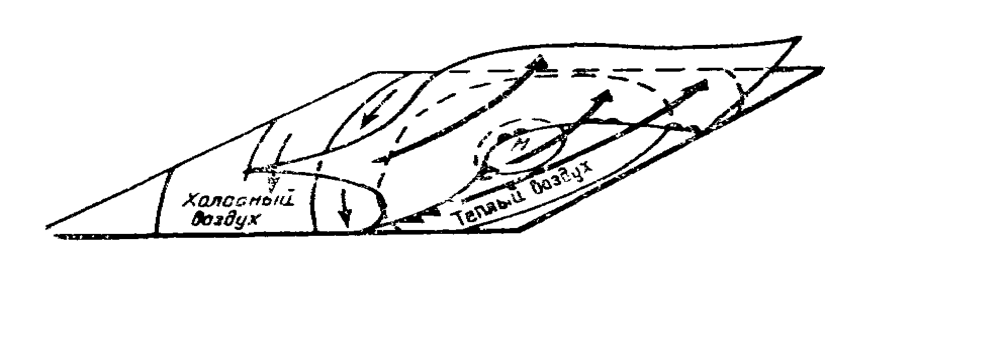
\includegraphics[scale=1]{13_cyclon_model.pdf}
   \caption{Пространственная модель молодого циклона}
   \label{fig:cyclon_model}
\end{figure*}

На рис.~XX вверху и внизу даны два вертикальных разреза через область
циклона. Верхний сделан к северу от центра циклона, нижний "--- к югу и
пересекает все три рассмотренные зоны. На нижнем виден подъём тёплого
воздуха в передней части циклона над поверхностью тёплого фронта и
образование характерной облачной системы, а также распределение
течений и облаков у холодного фронта в тыловой части циклона. Верхний
разрез пересекает поверхность основного фронта только в свободной
атмосфере; у земной, поверхности и здесь лишь холодный воздух, тёплый
течёт над ним. Разрез проходит через северный край области фронтальных
осадков.

Изменение направления ветра при движении по линии АВ и CD видно из
рис. XX, где показаны линии тока холодного и тёплого воздуха.

Тёплый воздух в молодом циклоне движется быстрее, чем перемещается
само возмущение. Поэтому через возмещение протекает все новый и новый
тёплый воздух, опускающийся по холодному клину в тылу циклона и
восходящий в его передней части.

С ростом амплитуды возмущения тёплый сектой циклона суживается:
холодный фронт постепенно нагоняет медленно движущийся тёплый и
наступает момент, когда тёплый и холодный фронты циклона смыкаются.

Центральная область циклона у земной поверхности вся заполняется
холодным воздухом, а тёплый воздух оттесняется в более высокие слои.

\section{Опасные и особо опасные для ВМФ явления}
\label{sec:dangerous}

\subsection{Опасные явления}

\textbf{Опасным} для Военно-Морского Флота метеорологическим явлениям
(ОЯ) называется такое явление, которое затрудняет или исключает
действие сил, применение оружия и использование технических средств
ВМФ или может нанести материальный ущерб.

\subsection{Особо опасные явления}

\textbf{Особо опасным} для ВМФ метеорологическим явлением (ООЯ)
называется такое явление, которое по своей интенсивности, времени
возникновения, продолжительности и площади распространения может
привести к срыву поставленных задач или значительному материальному
ущербу.

К опасным и особо опасным для ВМФ явлениям относятся те
метеорологические элементы и явления, которые по своей интенсивности,
продолжительности и площади распространения достигли критериев,
указанных в табл.~\ref{tab:dangerous}.

Перечень опасных и особо опасных явлений, их критерии и термины могут
уточняться гидрометеорологической службой флота (флотилии) в
зависимости от физико\-/географических особенностей зоны ответственности
флота (флотилии), а также тактико\-/технических данных кораблей (судов)
и техники ВМФ.

Прогноз опасного (ОЯ) или особо опасного (ООЯ) метеорологического
явления называется предупреждением.

Сообщение о начавшемся опасном или особо опасном метеорологическом
явлении называется оповещением.

\small
\begin{longtable}{l|c|c|c|c|c|c}
  \toprule[2pt]
  \multirow{7}{*}{\shortstack[l]{\textbf{Название} \\ \textbf{метеорологического явления} \\ вид \\ элемента}}
  & \multicolumn{3}{c|}{Опасные явления}
  & \multicolumn{3}{c}{Особо опасные явления} \\
  \cmidrule{2-4} \cmidrule{5-7}
  & \multirow{6}{*}{\begin{sideways}\shortstack{Интенсивность, \\ единица измерения}\end{sideways}}
  & \multirow{6}{*}{\begin{sideways}\shortstack{Продолжительность, \\ час}\end{sideways}}
  & \multirow{6}{*}{\begin{sideways}\shortstack{Площадь \\ распространения, \%}\end{sideways}}
  & \multirow{6}{*}{\begin{sideways}\shortstack{Интенсивность, \\ единица измерения}\end{sideways}}
  & \multirow{6}{*}{\begin{sideways}\shortstack{Продолжительность, \\ час}\end{sideways}}
  & \multirow{6}{*}{\begin{sideways}\shortstack{Площадь \\ распространения, \%}\end{sideways}}
  \\
  &\ &\ &\ &\ &\ &\ \\
  &\ &\ &\ &\ &\ &\ \\
  &\ &\ &\ &\ &\ &\ \\
  &\ &\ &\ &\ &\ &\ \\
  &\ &\ &\ &\ &\ &\ \\
  &\ &\ &\ &\ &\ &\ \\
  &\ &\ &\ &\ &\ &\ \\
  \midrule[2pt]
  \multicolumn{1}{c|}{1} & 2 & 3 & 4 & 5 & 6 & 7 \\
  \midrule[2pt]
  \endfirsthead
  \toprule[2pt]
  \multicolumn{1}{c|}{1} & 2 & 3 & 4 & 5 & 6 & 7 \\
  \midrule[2pt]
  \endhead
  
  \multicolumn{7}{l}{\textbf{Ветер}} \\*
  \multicolumn{7}{l}{\textit{для удалённых районов океанов и морей}} \\*
  средняя скорость & 12\otdo29\mps & любая & $\ge10$  &               &       &        \\*
  {}               & $\ge30$\mps   & любая & $\le30$  & $\ge30$\mps   & любая & $>30$  \\
  порывы           & 12\otdo34\mps &       & $\ge10$  &               &       &        \\*
  {}               & $\ge35$\mps   &       & $\le30$  & $\ge35$\mps   &       & $>30$  \\
  \midrule
  средняя скорость & 18\otdo34\mps & любая & $\ge10$  & $\ge35$\mps   &       &        \\*
  {}               & $\ge32$\mps   & любая & $\le10$  &               & любая & $>30$  \\
  порывы           & 18\otdo39\mps &       & $\ge10$  &               &       &        \\
  \midrule

  \multicolumn{7}{l}{\textbf{Шквал}} \\*
  максимальная скорость ветра
  {}               & 15\otdo29\mps & любая & любая    & $\ge30$\mps   & любая &$\ge10$ \\*
  {}               & $\ge30$\mps   & любая & $<30$    &               &       &        \\ 
  \midrule

  \multicolumn{7}{l}{\textbf{Обледенение кораблей, судов, отложение льда:}} \\*
  медленное        & $\le0,6$\,см/ч &      &          &               &       &         \\
  \midrule
  быстрое          &               &       &          & $0,7\div1,3$\,см/ч &  &         \\
  \midrule
  очень быстрое    &               &       &          & $\ge1,4$\,см/ч &      &         \\
  \midrule

  \multicolumn{7}{l}{\textbf{Осадки}} \\*
  дождь и дождь со снегом & 15\otdo49\,мм & $\le12$ & $\ge10$ & $\ge50$\,мм & $\le12$ & $>30$ \\
  \midrule
  снег             & $\ge50$\,мм   & $\le12$ & $\le30$ &               &      &         \\*
  {}               & 7\otdo19\,мм  & $\le12$ & $\ge10$ &               &      &         \\
  \midrule
  дождь ливневый   & $\ge20$\,мм   & $\le12$ & $\le30$ & $\ge20$\,мм  & $\le12$ & $>30$ \\*
  {}               &               &         &         & $\ge30$\,мм   & $\le1$ & $>30$ \\
  \midrule
  \textbf{Гроза}   & любая         &         & $\ge10$ &               &      &         \\
  \midrule

  \multicolumn{7}{l}{\textbf{Туман}} \\*
  видимость        & 500\otdo1000\,м & $>3$  & $\ge10$ &               &      &         \\*
  {}               & $<500$\,м     & $<12$   & $\le30$ & $<500$\,м    & $\ge12$ & $>30$ \\ 
  \midrule

  \multicolumn{7}{l}{\textbf{Метель (в том числе низовая)}} \\*
  \multicolumn{7}{l}{\textit{для побережий арктических и дальневосточных морей}} \\*
  скорость ветра   & 11\otdo14\mps & $>3$    & $\ge10$ &               &      &         \\*
  {}               & $\ge15$\mps   & $<12$   & $\le30$ & $\ge15$\mps  & $\ge12$ & $>30$ \\
  \midrule
  скорость ветра   & 11\otdo24\mps & $>3$    & $\ge10$ &               &      &         \\*
  {}               & $\ge25$\mps   & $<12$   & $\le30$ & $\ge25$\mps  & $\ge12$ & $>30$ \\*
  \midrule

  \multirow{2}{*}{\textbf{\shortstack{Гололёд (в том числе \\ сложные отложения)}}}
                   & 6\otdo19\,мм  & любая   & $\ge10$ &               &      &         \\*
  {}               & $\ge20$\,мм   & любая   & $\le30$ & $\ge20$\,мм   & любая & $>30$  \\
  \midrule

  \textbf{Изморозь} & $>50$\,мм    & любая   & $\ge10$ &               &      &         \\
  \midrule

  \textbf{\shortstack[l]{Изменение максимальной \\ или минимальной температуры \\ при переходе через 0\grC}}
                   & $\ge5$\grC    & $\le24$ & $>30$   &               &      &          \\
  \midrule

  \textbf{\shortstack[l]{Глубокий циклон \\ средних широт, \\ ураган}} & & & & \shortstack{наличие в \\ районе} & & \\       
  \midrule

  \textbf{\shortstack[l]{Тропический циклон, \\ тайфун}} & & & & \shortstack{наличие \\ в районе} & & \\
  
  \bottomrule[2pt]
  \caption{Опасные и особо опасные для ВМФ явления}
  \label{tab:dangerous}
\end{longtable}
\normalsize

\chapter{Основная терминология уточнения прогнозов погоды}

Под \textbf{прогнозом метеорологической обстановки}\index{прогноз
  погоды} (прогнозом погоды) понимается научно обоснованное
предсказание значений метеорологических элементов и явлений на
определённый район и заданный промежуток времени.

Прогноз является конечным результатом \textit{анализа атмосферных
  процессов}, который проводится на основе \textit{данных о
  фактической метеорологической обстановке} и известных
\textit{физических закономерностей} в развитии атмосферных процессов.

В краткосрочные прогнозы общего назначения включаются характеристики и
значения следующих метеорологических элементов и явлений:
\textbf{ветер}, \textbf{видимость}, \textbf{метеорологические
  явления}, \textbf{облачность}, \textbf{температура воздуха}.

Текст краткосрочных прогнозов должен быть кратким и ясным, не
допускающим двойственного толкования.

\section{Время}
\label{sec:time}

Под сроком действия прогноза метеорологической обстановки понимается
промежуток времени от начала действия прогноза до его окончания. По
времени действия прогнозы метеорологической обстановки подразделяются
на краткосрочные прогнозы, срок действия которых составляет от
нескольких часов до 1\otdo2~суток, и прогнозы малой заблаговременности
"--- от 3~до 5\otdo7~суток.

По требованию командования составляются прогнозы на короткий период
или промежуток времени продолжительностью до 5\otdo7~суток. На больший
срок составляются ориентировочные прогнозы или используются данные
наблюдений за многолетний период, климатические описания.

При детализации прогноза по времени используются термины: \textit{<<от
  (с) \ldots до \ldots ч>>}, \textit{<<утром>>} (06\otdo10~ч),
\textit{<<днем>>} (10\otdo18~ч), \textit{<<вечером>>} (18\otdo22~ч,
\textit{<<ночью>>} (22\otdo06~ч), \textit{<<в начале (середине, конце)
  срока>>}, \textit{<<в течение (до) первой (второй) половины суток
  (дня, ночи)>>}. \textbf{Началом срока} в прогнозе на сутки считаются
первые 8~ч, \textbf{серединой срока} "--- последующие 8~ч и
\textbf{концом срока} "--- последние 8~ч. В прогнозе на 12~ч "---
соответствующие 4-часовые периоды.

Если в прогнозе не даётся уточнение времени, то считается, что явление
наблюдается не менее 2/3~срока действия прогноза.

Использование в прогнозе термина \textbf{<<временами>>} означает, что ожидается
явление продолжительностью не более половины срока, на который
составляется прогноз.

Использование в прогнозе термина \textbf{<<времени>>} означает, что ожидается
явление продолжительностью не более половины срока, на который
составляется прогноз.

\textbf{Первая половина срока} "--- первые 12~часов с начала действия прогноза.

\textbf{Вторая половина срока} "--- вторые 12~часов с начала действия прогноза.

\textit{Для прогноза на последующие двое суток.}

\textbf{Первая половина срока} "--- первая половина прогнозируемого периода.

\textbf{Вторая половина срока} "--- вторая половина прогнозируемого периода.

\textbf{Начало срока} "--- первые 12~часов прогнозируемого периода.

\textbf{Конец срока} "--- последние 12~часов прогнозируемого периода.

\textbf{Середина срока} "--- последние 6~часов первой половины прогнозируемого
периода и первые 6~часов второй половины прогнозируемого периода.

\section{Ветер}
\label{sec:wind_p}

\textbf{Направление ветра} (откуда дует) указывается одним из восьми
румбов русскими названиями (\textit{северный}, \textit{северо-восточный}, \textit{южный} или
соответственно \textit{С}, \textit{СВ}, \textit{Ю} и т.\,д.).
Когда прогнозируется изменение
направления ветра на два румба и более, применяется термин \textit{<<с
переходом на \ldots>>}. Если ожидается колебание направления ветра в
пределах двух румбов, то в прогнозе указываются оба румба. Разрешается
употреблять термин \textit{<<ветер переменный>>} в случаях, когда направление
ветра будет изменяться в пределах 3~румбов и более, а скорость ветра
по району и пункту не будет превышать 10~и 8\mps соответственно.

Скорость ветра указывается в любой градации с интервалом не более 5\mps.

При скорости ветра 5\mps и менее указывается \textit{<<ветер слабый>>}. Если
ожидается резкое изменение скорости ветра или ветер с порывами, то
применяются термины: \textit{<<с усилием (ослаблением) до \ldots м/с>>}, \textit{<<порывы до
\ldots\mps>>}. При порывах указывается максимальная скорость ветра, которая
даётся одним числом с прибавлением \textit{<<до \ldots>>}.

Допускается применение термина \textit{бриз}.  Разрешается употребление
терминов \textit{шторм} и \textit{ураган} с обязательным указанием скорости
ветра 21\mps и~более и~30\mps и~более соответственно.

При прогнозировании ветра указывается время согласно п.\ref{sec:time}.

Примеры:
\begin{enumerate}[label={}]
\item Ветер Ю, слабый.
\item Ветер С, СВ 4--7\mps.
\item Ветер ЮЗ 6--9\mps, с усилением днем до 9--12\mps.
\item Ветер Ю 9--12\mps, в конце срока 5--8\mps.
\item Ветер СЗ 6--9\mps, в середине срока порывы до 17\mps.
\item Ветер ЮЗ 5--10\mps, ночью переменный слабый.
\item Ветер СЗ, С 10--12\mps, днем порывы до 19\mps.
\item Ветер ЮЗ, с переходом от 13 до 16 ч на СЗ 7--10\mps.
\item Ветер ЮЗ, с переходом в середине срока на СЗ 7--10\mps.
\item Ветер СВ 8--12\mps, в конце маршрута ЮВ 15--18\mps.
\item Ветер С, СВ, с переходом утром на З, ЮЗ 12--15\mps и усилением (ослаблением) до 15--20\mps (6--8\mps).
\end{enumerate}

В прогнозах погоды направление ветра указывается в \textbf{четвертях
  горизонта} (слово четверть не пишется). Ветер указанного направления
может изменяться в пределах соответствующей четверти. Например, термин
\textit{<<ветер юго-западный>>} означает, что в течение
прогнозируемого промежутка времени направление ветра должно
сохраняться в пределах от 270 до 180\gr.

\section{Видимость}
\label{sec:visibility}

\textbf{Горизонтальная видимость} указывается независимо от того,
прогнозируются или не прогнозируются явления, ухудшающие видимость.

Видимость указывается в километрах и метрах в следующих градациях:
более 10~км, 4\otdo10~км, 2\otdo4~км, 1\otdo2~км, 1000~м и менее.

В прогнозе видимость по возможности может даваться в градациях
500-1000 и менее 5000 м.

При прогнозировании явлений погоды, ухудшающих видимость, указывается
ожидаемая минимальная горизонтальная видимость в этих
явлениях. Разрешается применение терминов <<в явлениях>>,
<<в явлении>>.

Если за время действия прогноза видимость будет более 5~миль, то в
прогнозе указывается: <<видимость хорошая>>.

В явлениях (снежные заряды, снег, морось, дождь и т.д.) указывается
ухудшение видимости до 1\otdo2~миль, 5\otdo10~кбт. Или менее
5~кбт. Указанная видимость будет сохраняться только во время действия
явления. При прекращении указанного явления видимость будет
улучшаться.

Примеры:
\begin{enumerate}[label={}]
\item Видимость 10~км, в дымке 4--10~км.
\item Дымка, утром туман. Видимость 4--10~км, в тумане менее 500~м.
\item Дымка, кратковременные осадки. Видимость 4--10~км, в явлениях 2--4~км.
\end{enumerate}

\begin{longtable}{p{0.2\textwidth}|p{0.7\textwidth}}
  \toprule
  Термин & Применение термина \\
  \midrule
  \endfirsthead
  \toprule
  Термин & Применение термина \\
  \midrule
  \endhead
  Туман
         & Видимость 1000~м и менее на площади более 30\% \\
  \midrule
  Местами туман (утром, вечером, ночью)
         & Видимость 1000~м и менее в отдельных частях района \\
  \midrule
  Гроза
         & Явление охватывает более 50\% площади \\
  \midrule
  Местами гроза
         & Грозы ожидаются местами в различных частях района (менее 50\%) независимо от их частоты и интенсивности \\
  \midrule
  Метель
         & При снегопаде и скорости ветра более 10 м/с, когда явление ожидается на площади более 50\% \\
  \midrule
  Местами метель
         & Явление ожидается на отдельных гидрометеостанциях (постах) при снегопаде и кратковременных усилениях ветра более 10 м/с \\
  \midrule
  Гололёд
         & Явление ожидается на площади более 10\% \\
  \midrule
  Обледенение
         & Явление ожидается в любой части района \\
  \bottomrule
  \caption{Применение терминов видимости}
\end{longtable}

\section{Облачность}
\label{sec:clouds_p}

\textbf{Облачность} прогнозируется с указанием общего количества и
высоты нижней границы облаков нижнего яруса. В прогнозе рекомендуется
давать характеристику облаков.

Количество облачности указывается в любой градации с интервалом не
более 3~баллов\footnote{Детальные характеристики облачности даются в
  прогнозах специального назначения}.

В прогнозах погоды облачность указывается в баллах, что означает:
0\otdo3~балла "--- ясно; 3\otdo5~баллов "--- небольшая облачность;
5\otdo7~баллов "--- умеренная облачность; 7\otdo9~баллов "---
значительная облачность; 9\otdo10~баллов "--- сплошная облачность.

Термин \textit{переменная облачность} "--- означает, что за время
действия прогноза количество облачности несколько раз должно
изменяться от 0\otdo3~баллов до 9\otdo10~баллов.

Термин \textit{облачность верхнего и среднего ярусов} "--- означает,
что должны наблюдаться облака высотой 2~км. Прогнозируется количество
облаков только среднего и нижнего ярусов.

При облачности от 0 до 3 баллов употребляется термин
\textit{безоблачно} или \textit{малооблачно}. Когда метеорологическая
обстановка приводит к изменению количества облаков в интервале более
3~баллов, то применяются термины \textit{<<облачность \ldots баллов с увеличением
(уменьшением) до \ldots баллов>>} или \textit{<<облачность \ldots баллов с разрывами
(прояснениями) до \ldots баллов>>}.

Для характеристики облаков верхнего и среднего ярусов указывается
\textit{<<облачность верхнего (среднего) яруса}>> или
\textit{<<облачность верхняя (средняя)>>} без указания её количества и
форм облаков.

Если ожидаются облака нескольких ярусов (слоев), допускается
употребление термина \textit{<<облачность многослойная>>} но с
указанием, по возможности, формы облаков нижнего яруса, их количества.

В прогнозе по пункту (базе) дополнительно указывается форма облаков
нижнего яруса. Форма облаков нижнего яруса даётся полными русскими
названиями (не более 2 основных форм).

Высота нижней границы облаков указывается в любой градации через 100~м
до высоты 300~м, через 300\otdo400~м до высоты 1000~м и через 500\otdo1000~м
при высоте нижней границы облаков более 1000~м.

Примеры:
\begin{enumerate}[label={}]
\item Малооблачно, днем 4--7 баллов кучевых форм, высотой 1000--1500~м.
\item Безоблачно, в конце срока облачность верхнего яруса.
\item Облачность 9--10 баллов, многослойная, 4--7 баллов разорванно-дождевой, высотой 150--250~м.
\item Облачность 9--10 баллов, временами 3--5 баллов, многослойная, слоистых форм, разорванно-дождевая, высотой 200--3000~м.
\item Облачность 5--8 баллов, средняя, слоисто-кучевая, высотой 500--800~м.
\item Облачность 7--10 баллов, слоисто-дождевая, высотой 200--300~м.
\item Облачность 6--9 баллов, кучево-дождевая, высотой 600--1000~м.
\item Облачность 5--7 баллов, средняя, верхняя.
\item Облачность 10 баллов, многослойная, слоисто-дождевая, высотой 200--300~м.
\end{enumerate}

\begin{longtable}{p{0.2\textwidth}|p{0.7\textwidth}}
  \toprule
  Термин & Применение термина \\
  \midrule
  \endfirsthead
  \toprule
  Термин & Применение термина \\
  \midrule
  \endhead
  Ясно или безоблачно
         & Преобладает ясная погода или имеется облачность до 3 баллов облаков всех ярусов \\
  \midrule
  Малооблачная погода (небольшая облачность)
         & Облачность 3\otdo5 баллов нижнего яруса, 4\otdo7 баллов среднего яруса или 5\otdo8 баллов верхнего яруса \\
  \midrule
  Переменная облачность \footnote{Термины относятся к облакам нижнего яруса и плотным облакам среднего яруса}
         & Облачность 3\otdo8 баллов или может меняться от 1\otdo3 до 6\otdo9 баллов \\
  \midrule
  Облачная погода с прояснениями
         & Облачность меняется от 8\otdo10 до 1\otdo3 баллов \\
  \midrule
  Облачная погода (значительная облачность)
         & Облачность 7\otdo10 баллов \\
  \midrule
  Сплошная облачность
         & Преобладание облачности 10 баллов с возможными отдельными уменьшениями до 7 баллов \\
  \bottomrule
  \caption{Применение терминов облачности}
\end{longtable}

\section{Метеорологические явления}
\label{sec:meteo_phenom}

В прогноз включаются следующие явления: осадки (дождь, снег), туман,
дымка, парение моря, гроза, обледенение кораблей и судов, гололёд,
изморозь, град, метель.

Гололёд, изморозь, град указываются только для береговых районов,
метель указывается для береговых районов и для районов с неподвижным
льдом.

Термин \textit{осадки} употребляется, когда прогнозируемая температура
воздуха колеблется в пределах от 0 до $\pm3\grC$, в остальных случаях
обязательно указывается вид осадков (фазовое состояние): дождь, снег,
морось, град и др.

Когда ожидается безоблачная или малооблачная погода, то термин
\textit{без осадков} в прогнозе опускается. Применение термина
\textit{прекращение осадков} обязательно с указанием времени их
ожидаемого прекращения.

При прогнозировании осадков термин \textit{кратковременный}
применяется, если ожидаются осадки продолжительностью не более 3~ч за
половину суток.

При зарядах используется термин \textit{<<снег (осадки) зарядами>>}.

В прогнозах интенсивность грозы не указывается.

В прогноз включаются и местные явления, например \textit{бора}.

Примеры:
\begin{enumerate}[label={}]
\item \ldotsкратковременный снег.
\item \ldotsкратковременный сильный дождь.
\item \ldotsкратковременные слабые осадки.
\end{enumerate}

\section{Температура воздуха}
\label{sec:temp}

Указывается ожидаемая температура воздуха (минимальная ночью и
максимальная днем) с интервалом 3\grC для пунктов экваториальных и
тропических районов океанов и с интервалом 5\grC, по другим районам
океанов и морей.

Если ожидаемая температура воздуха по району океана или моря не
укладывается в 3 или 5\grC, то следует выделять части района, где
температура отличается от основного ожидаемого фона.

Когда в течение суток ожидается аномальный суточный ход температуры,
то это даётся в прогнозе с применением терминов \textit{повышение} или
\textit{понижение} и указанием времени, когда ожидается это изменение.

Пример: Температура воздуха 15--17\grC, в конце срока понижение до
9--11\grC.

При колебании температуры воздуха от 1 до $-1\grC$ употребляется
термин \textit{<<около 0\gr{}C>>}.

\chapter{Составление прогноза погоды}

\section{Общие принципы составления прогноза погоды и основные прогностические методы}

Основная идея прогноза различных метеорологических элементов и явлений
заключается в предположении, что с перемещением воздушных масс и
фронтов переносятся и свойственные им условия погоды. Поэтому за
исходные значения метеорологических элементов принимают их значения в
том районе, откуда ожидается перемещение воздушной массы или фронта в
район, для которого составляют прогноз погоды.

К исходным значениям метеорологических элементов вводят поправки на
изменение условий погоды в связи с трансформацией воздушной массы и
эволюцией фронта, а также на суточный ход метеорологических элементов.

Для прогноза количественных характеристик метеорологических элементов
по пути следования судна достаточно снять соответствующие значения
этих метеоэлементов с карты, считая, что за 6\otdo12~ч не произойдет
больших изменений.

Прежде, чем дать прогноз погоды, делается прогноз синоптического
положения (прогноз развития атмосферных процессов), сущность которого
заключается в том, что на основе анализа синоптических карт
прогнозируется положение основных синоптических объектов на
интересующее нас время и возможные их изменения.

При прогнозировании синоптического положения руководствуются тремя принципами:
\begin{enumerate*}[itemjoin={{; }}, label={\arabic*)}]
\item принцип инерционности метеорологических процессов
\item принцип экстраполяции
\item принцип физических заключений
\end{enumerate*}

\textbf{Принцип инерционности}\index{принцип инерционности} состоит в
том, что синоптические процессы развиваются не мгновенно, а на
протяжении определенного времени, следовательно, в течение какого-то
отрезка времени сохраняется более или менее стационарное состояние
синоптических объектов. Например, циклон не появляется и не исчезает
мгновенно, а развивается некоторое время. Поэтому, если прогноз
делается на короткое время, инерционность играет очень важную
роль. Можно считать, что существующие синоптические объекты не
изменятся, а только соответственно переместятся, т.\,е. учитывается их
инерционность. Если прогноз делается на длительный период, то принцип
инерционности один не достаточен.

\textbf{Принцип экстраполяции}\index{принцип экстраполяции}
заключается в том, что на основании развития атмосферных процессов
устанавливаются скорости и ускорения в развитии синоптических объектов
и их перемещения. Принцип экстраполяции состоит, прежде всего, в
\textit{установлении тенденции развития} синоптических объектов и
экстраполяции развития их на прогнозируемый промежуток времени.

\textbf{Принцип физических заключений}\index{принцип физических
  заключений} состоит в том, что на основе знаний законов развития
синоптических объектов устанавливаются возможные изменения их, а также
вероятность появления новых синоптических объектов, т.\,е. учитываются
физические закономерности развития синоптических объектов.

Основой прогноза погоды является прогноз синоптического положения
(имеется ввиду, что погода переносится вместе с синоптическими
объектами). Но необходимо учитывать изменения погодных характеристик
при перемещении и развитии синоптических объектов. Таким образом,
анализируя синоптические объекты, прогнозирование погоды необходимо
делать не по отдельным элементам, а в комплексе.

\textbf{Прогноз перемещения барических систем и фронтов}\index{прогноз
  перемещения}. В практике прогноза применяется ряд способов
определения перемещения барических центров и фронтов и их
эволюции. Для получения более надежных результатов обычно используют
не один какой-либо способ, а несколько, что гарантирует от грубых
просчетов.

Наиболее простой способ определения перемещения барических центров и
осей "--- способ прямолинейной и криволинейной экстраполяции.

\textbf{Прямолинейная экстраполяция}\index{прямолинейная интерполяция}
заключается в определении направления и скорости перемещения
барического центра (или фронта) за предыдущий промежуток времени с
помощью двух синоптических карт, в предположении, что такое же
направление и скорость сохранятся и на срок прогноза. Обычно
определяют направление и величину перемещения за 6, 12 или 24~ч.

\textbf{Криволинейная экстраполяция}\index{криволинейная
  экстраполяция} позволяет уточнить расчет направления и скорости
перемещения синоптического объекта, предполагая постоянной не
скорость, а ускорение, которое определяется по изменению направления и
скорости перемещения за два промежутка времени, т.\,е. по трем картам
погоды.

Оси ложбин (или фронты, оси гребней) перемещаются в направлении
нормали к ним, но с неодинаковой скоростью в различных частях. В связи
с этим их направление и скорость должны быть определены не менее чем
для двух -- трех точек.

Линейная экстраполяция применима на сроки прогноза не более 6\otdo12~ч,
тогда как криволинейная экстраполяция при отсутствии резких изменений
синоптического положения часто дает удовлетворительный результат и на
срок прогноза 12\otdo24~ч.

Помимо прямолинейной и криволинейной экстраполяции, прогноз
перемещения атмосферных фронтов может быть осуществлен на основе
расчета нормальной составляющей скорости геострофического ветра у
земной поверхности. Однако следует учитывать, что циклон может
углубляться или заполняться, в связи с чем меняются расстояния между
изобарами, а следовательно, скорость ветра и скорость перемещения
фронтов.

Прогноз перемещения барических систем может быть осуществлен и по
изаллобарическому полю. Для этого пользуются следующими правилами,
вытекающими из теоретических исследований и опыта:
\begin{enumerate}[label={\textbullet~}]
\item циклоны (антициклоны) с круговыми изобарами перемещаются в
  направлении на центр падения (роста) давления;
\item циклоны (антициклоны) с изобарами, вытянутыми в виде эллипса,
  перемещаются между направлением на центр падения (роста) давления и
  большой осью изобар, причем, чем сильнее вытянут эллипс, тем ближе к
  последней;
\item скорость перемещения циклона (антициклона) прямо пропорциональна
  алгебраической разности барических тенденций в изаллобарических
  центрах;
\item циклон перемещается параллельно прямой, соединяющей центры
  связанных с ним областей роста и падения давления, если эти области
  одинаковы по интенсивности;
\item начавшееся удаление области падения (роста) от центра циклона
  (антициклона) в переднюю часть барической системы и ослабление этой
  области являются признаком замедления перемещения этих барических
  образований;
\item барическая система стационарна, когда распределение барических
  тенденций вблизи ее центра одинаково по всем направлениям от центра
  (так будет, например, если центр области падения или роста давления
  совпадает с барическим центром).
\end{enumerate}

\textbf{Направление перемещения циклона}\index{направление перемещения
  циклона} может быть определено по правилам, вытекающим из свойств
ведущего потока "--- устойчивого воздушного течения на высоте 4\otdo6~км.
Согласно этим правилам, циклон перемещается параллельно
направлению изобар хорошо выраженного теплого сектора таким образом,
что холодный воздух остается слева. Скорость движения циклона примерно
равна скорости ветра в теплом секторе.

При составлении прогноза перемещения фронтов можно использовать
следующие правила:
\begin{enumerate}[label={\textbullet~}]
\item фронт перемещается тем быстрее, чем меньше расстояние между
  изобарами вдоль линии фронта;
\item при развитии (углублении) циклона увеличивается барический
  градиент, усиливается ветер, увеличивается скорость перемещения
  фронта; при заполнении циклона барический градиент уменьшается,
  ветер ослабевает и скорость перемещения фронта снижается;
\item скорость перемещения фронта (ложбины) прямо пропорциональна
  алгебраической разности барических тенденций по обе стороны от
  фронта (ложбины); при увеличении этой разности фронт перемещается
  быстрее, при уменьшении "--- медленнее.
\end{enumerate}

\textbf{Прогноз эволюции барических систем и фронтов}\index{прогноз
  эволюции барических систем и фронтов}. При составлении прогноза
эволюции барических образований следует определить, в какой стадии
развития находится барическое образование, и, исходя из этого,
установить ее последующую стадию. При этом надо изучить предшествующую
историю развития барического образования хотя бы за предшествующие
24~ч. Аналогично, составляя прогноз эволюции атмосферных фронтов,
нужно выявить, насколько лучше или хуже. выраженным становится фронт в
полях метеорологических элементов от одного срока, наблюдений к
другому, и установить причины усиления или ослабления фронтальных
явлений погоды.

\textbf{Обострение}\index{фронт!обострение} или
\textbf{размывание}\index{фрони!размывание} атмосферных фронтов может
быть определено по изменению контраста температуры на фронте, так как
в большинстве случаев увеличение этого контраста сопровождается
обострением фронта (увеличением количества облачности и ее
вертикальной мощности и т.\,д.), а уменьшение разности температур
воздушных масс, разделяемых фронтом, как правило, приводит к улучшению
условий погоды в зоне фронта.

Об углублении или заполнении циклонов, усилении или ослаблении
антициклонов судят по барической тенденции в их центрах, которая
характеризует не только эволюцию, но и скорость последней. На этом
основаны следующие правила тенденций:

\begin{enumerate}[label={\textbullet~}]
\item циклон углубляется (заполняется), если в его центре наблюдаются
  отрицательные (положительные) тенденции;
\item антициклон усиливается (ослабевает), если в его центре
  наблю-даются положительные (отрицательные) тенденции;
\item близкие к нулевым тенденции в центре барических систем говорят о
  том, что их глубина существенно изменяться не будет;
\item барическая ложбина углубляется (заполняется), когда нулевая
  изотенденция проходит позади (впереди) оси ложбины;
\item барический гребень усиливается (ослабевает), когда нулевая
  изотенденция проходит позади (впереди) оси гребня;
\item при отрицательных (положительных) тенденциях в центре циклона
  (антициклона) продолжительность его углубления (усиления) будет тем
  больше, чем дальше от центра циклона (антициклона) в его тылу
  проходит нулевая изотенденция;
\item удаление области падения (роста) от центральной части циклона
  (антициклона) на его периферию указывает на быстрое заполнение
  циклона и ослабление антициклона.
\end{enumerate}

Прогноз условий погоды для движущегося судна осложняется тем, что
приходится учитывать перемещение не только воздушных масс, барических
образований, фронтов и т.\,д., но и перемещение судна. Иными словами,
необходимо найти перемещение судна относительно движущихся
объектов. Эта задача решается методами, используемыми при расчете
маневрирования кораблей.

Решение удобнее всего вести на генеральной карте, для чего на нее с
синоптической карты по координатам необходимо перенести характерные
объекты синоптического положения (центры барических систем, фронты и
т.\,п.) в районе предстоящего плавания судна.

\begin{figure*}[htb]
   \centering
   
\includegraphics[scale=3]{14_move_ship_a.eps}
   \caption{Расчет перемещения судна относительно движущейся барической системы}
   \label{fig:move_ship}
\end{figure*}

Пусть в начальный момент центр циклона располагается в точке $H$, а
судно — в точке $K$. Циклон перемещается в направлении $HH'$ со скоростью
$\vec{V}_H$, а судно следует курсом $KK'$ со скоростью $\vec{V}$. В первом приближении
примем, что все части циклона движутся так же, как и его центр.

При решении задач на относительное перемещение принято один из
объектов считать неподвижным, тогда второй объект движется
относительно неподвижного со скоростью $\vec{V}_\rho$, равной
векторной сумме скоростей маневрирующих объектов
($\vec{V}_\rho = \vec{V}_H + \vec{V}$) "--- в данном случае за
неподвижный объект удобнее принять циклон.

Построим у центра циклона в произвольном масштабе треугольник
скоростей. Для этого от точки $H$ отложим векторы $\vec{V}_H$ и
$\vec{V}$. Вектор $V_\rho$, замыкающий их, и есть вектор относительной
скорости. Проведем относительный курс "--- линию $KK_\rho$,
параллельную вектору $\vec{V}_\rho$. Именно по этой линии со скоростью
$V_\rho$, перемещается судно относительно циклона.

Отложив по линии $KK_\rho$ в масштабе карты отрезки, которые судно
пройдет за 3, 6, 9~ч, получим картину перемещения судна относительно
циклона. Следует помнить, что, перемещаясь по линии $KK_\rho$, судно
остается на прежнем истинном курсе. Так, из рисунка видно, что
приблизительно через 12~ч оно пересечет линию теплого фронта и при
этом ветер резко перейдет от носовых курсовых углов к траверзным. В
этот момент фактическое место судна будет в точке $A$, а не в точке
$B$, и фронт будет занимать фактическое положение, показанное на
рисунке пунктиром.

\section{Порядок составления прогноза погоды}

Для составления прогноза погоды необходимо определить в какой
воздушной массе в настоящее время находится наблюдатель, какая
воздушная масса приближается к месту наблюдения, какова подвижность
воздушных масс. Для этого необходимо произвести измерение температуры,
давления, влажности воздуха, определить величину барической тенденции,
форму и количество облаков. При этом необходимо учитывать суточный ход
основных метеоэлементов.

\section{Предсказание погоды по местным признакам}

В случае если прогноз погоды по радио не был принят, единственным
источником информации об ожидаемой погоде являются местные признаки "---
\textit{это такие явления и изменения в ходе метеорологических элементов,
наблюдаемые и измеряемые в одном пункте, на основании которых можно
сделать заключение о предстоящем характере погоды.}

Вместе с тем, по радио передается прогноз на обширный район, который в
отдельных точках может не соответствовать действительности, поэтому в
море необходимо постоянно наблюдать за метеорологической обстановкой и
уточнять прогноз погоды по местным признакам.

Местные признаки основаны на многолетнем опыте и изучении воздушных
масс, фронтов и барических систем. Знание их позволяет судоводителю
предсказывать погоду. Однако в настоящее время местные признаки в
основном используются для уточнение прогноза, полученного по
радио. Вместе с тем в полученных прогнозах могут быть существенные
ошибки, поэтому судоводитель должен постоянно наблюдать за
метеорологической обстановкой, чтобы вовремя уточнить прогноз.

На судах, где не принимают по радио прогноз погоды, местные признаки
являются единственным средством для определения ожидаемых изменений
погоды.

Составляя прогноз погоды по местным признакам, или используя их для уточнения прогноза, полученного по радио, необходимо провести следующие операции:

\begin{enumerate}[label={\arabic*.~}]
\item выполнить анализ метеорологических наблюдений. При этом
  наблюдаемые явления погоды должны быть объяснены и их изменения
  увязаны с развивающимися в данное время процессами;
\item определить, в какой воздушной массе, а также в какой части
  барической системы или перед каким фронтом находится судно;
\item выяснить, не наблюдались ли оптические и другие явления,
  служащие признаком приближения того или иного фронта:
\item по выявленным признакам определить, какая погода придет на смену
  существующей.
\end{enumerate}

При составлении прогноза погоды по местным признакам необходимо иметь в виду следующие общие правила:

\begin{enumerate}[label={\textbullet~}]
\item чем больше признаков указывает на изменение или сохранение
  погоды, тем большая надежность прогноза;
\item один какой-нибудь признак не всегда является безусловным
  предвестником того или иного явления;
\item если несколько признаков противоречат друг другу, то следует
  ожидать неустойчивой погоды;
\item чем медленнее происходит изменение явления, наблюдаемого в
  качестве местного признака, тем медленнее будет происходить
  изменение погоды и тем продолжительнее она будет.
\end{enumerate}

После анализа данных синоптической консультации с учетом изложенных
выше положений приступают к \textbf{анализу своих корабельных
  наблюдений}\index{анализ наблюдений}. Для этого необходимо иметь
данные за 6\otdo8 сроков наблюдений, равномерно распределенных в течение
суток. Эти данные должны быть обработаны и занесены в специальный
журнал. Имея такие наблюдения, прежде всего, необходимо сопоставить
ход атмосферного давления с изменением направления, силы и характера
ветра. Это позволяет ориентироваться в барическом поле. Так, например,
если при низком стоянии барометра давление воздуха понижается и ветер
меняется с южных на юго-западные румбы, то это указывает на движение
циклона с запада на восток севернее пункта наблюдения.

Правильный суточный ход метеоэлементов наблюдается в антициклоне, а
нарушение суточного хода будет характеризовать наличие циклоничности.



\backmatter{}

\printindex

\end{document}

%%% Local Variables:
%%% mode: latex
%%% TeX-master: t
%%% End:
